%% ****** Start of file apstemplate.tex ****** %
%%
%%
%%   This file is part of the APS files in the REVTeX 4 distribution.
%%   Version 4.1r of REVTeX, August 2010
%%
%%
%%   Copyright (c) 2001, 2009, 2010 The American Physical Society.
%%
%%   See the REVTeX 4 README file for restrictions and more information.
%%
%
% This is a template for producing manuscripts for use with REVTEX 4.0
% Copy this file to another name and then work on that file.
% That way, you always have this original template file to use.
%
% Group addresses by affiliation; use superscriptaddress for long
% author lists, or if there are many overlapping affiliations.
% For Phys. Rev. appearance, change preprint to twocolumn.
% Choose pra, prb, prc, prd, pre, prl, prstab, prstper, or rmp for journal
%  Add 'draft' option to mark overfull boxes with black boxes
%  Add 'showpacs' option to make PACS codes appear
%  Add 'showkeys' option to make keywords appear
\documentclass[aps,
prd,
amsmath,
amssymb,
twocolumn,
floatfix,
groupedaddress]{revtex4-1}
%\documentclass[aps,prl,preprint,superscriptaddress]{revtex4-1}
%\documentclass[aps,prl,reprint,groupedaddress]{revtex4-1}
\usepackage{graphicx}% Include figure files
%\usepackage{float}
%\usepackage{stfloats}
%\usepackage{fixltx2e}
\usepackage{placeins}
\usepackage{dcolumn}% Align table columns on decimal point
\usepackage{amsmath}
\usepackage{amsthm, amsfonts, amssymb}
%\usepackage{supertabular}
\usepackage{array}
\usepackage{times}
\usepackage{latexsym}
\usepackage{hyperref}
\hypersetup{backref,  
pdfpagemode=FullScreen,  
colorlinks=true,
linkcolor=red,
filecolor=red,
citecolor=blue}
\usepackage{epsfig}
\usepackage{subfigure}
% \usepackage{multicol}
%\usepackage{acronym}
%\usepackage[caption=false]{caption}
\usepackage{bm}% bold math


\newcommand{\Sum}{\displaystyle\sum\limits}
\newcommand{\Int}{\displaystyle\int\limits}
\newcommand{\ii}{{\rm i}}
\newcommand{\D}{\mathrm{d}}
\newcommand{\eff}{\mathrm{eff}}
\newcommand{\real}{\mathrm{real}}
\newcommand{\peak}{\mathrm{peak}}
\newcommand{\EOB}{\mathrm{EOB}}
\newcommand{\NR}{\mathrm{NR}}
\newcommand{\RD}{\mathrm{RD}}
\newcommand{\Olap}{\mathcal{O}}
\newcommand{\MM}{\mathrm{MM}}
\newcommand{\EFF}{\mathrm{EFF}}
\newcommand{\Y}{\mathrm{Y}}
\newcommand{\Z}{\mathrm{Z}}

\def\l({\left(}
\def\r){\right)}
%\def\l[{\left[}
%\def\r]{\right]}

\def\beq{\begin{equation}}
\def\eeq{\end{equation}}
\def\bea{\begin{eqnarray}}
\def\eea{\end{eqnarray}}
\def\nn{\nonumber}
\def\del{\partial}
\def\ola{\overleftarrow}
\def\ora{\overrightarrow}

% You should use BibTeX and apsrev.bst for references
% Choosing a journal automatically selects the correct APS
% BibTeX style file (bst file), so only uncomment the line
% below if necessary.
%\bibliographystyle{apsrev4-1}

\begin{document}

% Use the \preprint command to place your local institutional report
% number in the upper righthand corner of the title page in preprint mode.
% Multiple \preprint commands are allowed.
% Use the 'preprintnumbers' class option to override journal defaults
% to display numbers if necessary
%\preprint{}

%Title of paper
\title{Data Analysis with Effective-One-Body Waveforms}

% repeat the \author .. \affiliation  etc. as needed
% \email, \thanks, \homepage, \altaffiliation all apply to the current
% author. Explanatory text should go in the []'s, actual e-mail
% address or url should go in the {}'s for \email and \homepage.
% Please use the appropriate macro foreach each type of information

% \affiliation command applies to all authors since the last
% \affiliation command. The \affiliation command should follow the
% other information
% \affiliation can be followed by \email, \homepage, \thanks as well.
\author{some person1}
\email[]{prkumar@syr.edu}
%\homepage[]{Your web page}
%\thanks{}
%\altaffiliation{}
\affiliation{Department of Physics, Syracuse University}

\author{some person2}
%\email[]{prkumar@syr.edu}
%\homepage[]{Your web page}
%\thanks{}
%\altaffiliation{}
\affiliation{Department of Physics, Syracuse University}

%Collaboration name if desired (requires use of superscriptaddress
%option in \documentclass). \noaffiliation is required (may also be
%used with the \author command).
%\collaboration can be followed by \email, \homepage, \thanks as well.
%\collaboration{}
%\noaffiliation

\date{\today}

\begin{abstract}

% insert abstract here
\end{abstract}

% insert suggested PACS numbers in braces on next line
\pacs{}
% insert suggested keywords - APS authors don't need to do this
%\keywords{}

%\maketitle must follow title, authors, abstract, \pacs, and \keywords
\maketitle

\section{Introduction}\label{sec:level1:Introduction}
Investigating waveform models for use in searching for Stellar-Mass Black Hole Binaries (SMBHB).

\section{Objective}\label{sec:level1:Objective}
The following problems are tackled in this treatise:

\begin{itemize}
\item
In the most recent model to generate the gravitational waveform using the Effective-One-Body (EOB) approach \cite{BuonannoEOBv2Main}, the $\rho_{lm}$ resummation is used to calculate the rate of loss of Energy, which was originally introduced by \cite{DamourFluxhlm01}. 
\begin{equation}\label{eq:EDot01}
\frac{dE}{dt} = \frac{\hat{\Omega}^2}{8\pi} \displaystyle\sum\limits_{l}\displaystyle\sum\limits_{m} \left|\frac{\mathcal{R}}{M} h_{lm}\right|^2
\end{equation}
In the original prescription \cite{DamourFluxhlm01}, it was proposed to include the following set of $h_{lm}$ modes in calculating the rate of loss of energy using Eq.\eqref{eq:EDot01}: 
\begin{equation}
\{2\leq l\leq 6; 1\leq m \leq l\}
\end{equation}
Recent work\citep{BuonannoEOBv2Main}, with comparisons with more NR waveforms, suggests the use of the following set of $h_{lm}$ modes:
\begin{equation}
\{2\leq l \leq 7; (l-2)\leq m \leq l\}
\end{equation}
In either case, the summation runs over 20 and 17 modes, respectively. In the generation of the waveform, the calculation of the Energy flux is the most computationally expensive step. In order to make the waveform generation as computationally inexpensive as possible, we systematically search for the smallest set of $h_{lm}$ modes, which can be used to compute the Energy flux, and we still generate a waveform that is accurate enough. Accurate enough is defined here as having at least an overlap of 0.985 (or 0.995) with the waveform that uses a summation over all analytically known $h_{lm}$ modes to compute the Energy flux.
\item
The non-spinning EOB model has evolved a lot in the last few years, and the latest\citep{BuonannoEOBv2Main} has been tuned against a fair number of Numerical Relativity (NR) waveforms. With the increase in accuracy of the EOB model, its interesting to know how does it compare with Taylor time-domain and the Stationary Phase waveform models. As the EOB model employs various resummations to enforce convergence, for instance, for the multipolar waveform or the gravitational flux. We try to analyze how do the Taylor models compare with EOB. 
\item
The EOB waveforms have the ringdown stitched at the end, starting at the light-ring. We try to analyze the gain in signal-to-noise ratio because of having the ringdown attached to the inspiral-merger part of the waveform.
\item
Searches for gravitational waves in LIGO data have utilized a hexagonal placement metric \cite{SathyaMetric2PN} to place points in the component-mass space, such that one covers the space optimally. Optimality being defined as not losing more than a pre-specified amount of signal-to-noise ratio (SNR). Since this metric was constructed for 2PN frequency-domain waveforms, we analyze if this metric allows us to places points efficiently if one uses 3.5PN (or pseudo-4PN) waveforms?
\item
The latest non-spinning EOB model\citep{BuonannoEOBv2Main}, has been evolving for the past few years. The present model has been tuned against Numerical Relativity waveforms, and so we can expect it to be quite accurate in modeling the true gravitational waveforms. For a search that targets at detecting a gravitational-wave signal in LIGO data, it is not important if the mass-parameters that are recovered accurately follow the actual parameters. We try to find the part of the component-mass space, is it efficient to use the Stationary Phase or Taylor time-domain waveforms to detect gravitational wave signals. This is important because, the latter waveforms are much faster to generate than the EOB waveforms, and thus we could reduce the computational cost of the search by being able to use Stationary Phase waveforms, instead of EOB. 
\end{itemize}

\section{Waveform Models}\label{sec:level1:Waveform}
This section gives a brief summary of the construction of the non-adiabatic EOB waveforms and the adiabatic time-domain and frequency-domain Taylor waveforms. The Taylor waveforms use taylor series expansions for energy and energy flux from the binary from PN theory, and hence the name. The EOB waveform model employed here, is the most recently developed model \cite{BuonannoEOBv2Main} in literature. 

\subsection{Effective-One-Body Model}\label{sec:level2:Waveform:EOB}
The Effective-One-Body approach is the idea of mapping the two-body problem to a single body moving in a deformed Schwarzschild metric, which was originally proposed in Ref.\citep{EOBOriginalBuonannoDamour}. The model has seen several stages of development ever-since \cite{EOBdevel01,EOBdevel02,EOBNRdevel03,DamourFluxhlm01,EOBNRdevel01}.

The physical dynamics, in the effective-one-body mapping, is contained in the spacetime metric coefficients and the effective-one-body Hamiltonian \cite{EOBOriginalBuonannoDamour}. These crucial parts of the model, along-with the radiation-reaction force, i.e. the gravitational flux, can and have been tuned separately to model waveforms accurately \citep{EOBNRdevel01,DamourFluxhlm01,BuonannoEOBv2Main}.

Unlike the Taylor models, this model goes beyond the adiabatic limit, by incorporating the dynamics of the non-circular orbits beyond the innermost stable circular orbit. The particular EOB model we discuss here \citep{BuonannoEOBv2Main}, incorporates the non-adiabaticity with further accuracy by introducing non-quasi-circular corrections to the waveform.

\subsubsection{Dynamics}\label{sec:level3:Waveform:EOB:Dynamics}
Taking $m_1$ and $m_2$ as the masses of the two components of the binary system, we define $M = m_1 + m_2$, $\mu = m_1m_2/M$, $\eta = \mu/M$. The units used here are dimensionless, with $G = c = 1$. In polar coordinates $(r,\Phi)$, the EOB metric can be written as:
\begin{equation}
ds_{eff}^2 = -A(r)dt^2 + \dfrac{A(r)}{D(r)} dr^2 + r^2\left(d\Theta^2 + sin^2\Theta d\Phi^2\right)
\end{equation}
and, the effective EOB Hamiltonian reads:
\begin{equation}
\hat{H}_{eff} = \sqrt{A(r) \left( 1 +  \dfrac{A(r)}{D(r)}p_r^2 + 2(4 - 3\eta)\eta \dfrac{p_r^4}{r^2} + \dfrac{p^2_{\phi}}{r^2} \right)}\\
\end{equation}
It is found useful to reformulate the dynamics in terms of the momentum conjugate to the EOB \textit{tortoise} radial coordinate $(p_{r_*})$ be used, instead of the momentum conjugate to the radial coordinate $(p_r)$, in this formulation. In this coordinate, the evolution more regular close to the innermost stable circular orbit and beyond. 
\begin{equation}
\dfrac{dr_*}{dr} = \frac{\sqrt{D(r)}}{A(r)}
\end{equation}
The effective Hamiltonian then becomes \citep{BuonannoEOBv2Main}:
\begin{equation}
\hat{H}^{eff} = \sqrt{p^2_{r_*} + A(r) \left( 1 + 2(4 - 3\eta)\eta \dfrac{p_{r_*}^4}{r^2} + \dfrac{p^2_{\phi}}{r^2} \right)}
\end{equation}
and the real EOB Hamiltonian is given by:
\begin{equation}
\hat{H}^{real} = \dfrac{1}{\eta} \sqrt{1 + 2\eta (\hat{H}^{eff} - 1)} 
\end{equation}
The metric coefficients were originally calculated as Taylor expansions in  Refs.\cite{EOBOriginalBuonannoDamour,PadeAD}. At PN order $n$:
\begin{eqnarray}
A(r) = \Sum^{n+1}_{i=0} \dfrac{a_i (\eta)}{r^i},\quad
D(r) = \Sum^{n}_{i=0} \dfrac{d_i (\eta)}{r^i}\\
\end{eqnarray}
As suggested in Ref.\cite{PadeAD}, instead of the Taylor expansion for the metric coefficients, we use their Pade re-summations. This essentially enforces the existence of the EOB innermost stable circular orbit. For $A(r)$, we use Pade re-summation at order $(1,5)$, while for $D(r)$, we use the re-summation  at order $(0,3)$.
\begin{eqnarray}
D^0_3(r) &= \dfrac{r^3}{(52\eta - 6\eta^2) + 6\eta r + r^3}\\
A^1_5(r) &= \dfrac{\alpha_0 r^5 + \alpha_1 r^4}{\beta_0 r^5 + \beta_1 r^4 + \beta_2 r^3 + \beta_3 r^2 + \beta_4 r +\beta_5}\\
\end{eqnarray}
where, 
\begin{align*}
\alpha_0 &= 32 - 4a_4 - a_5 - 24\eta\\
\alpha_1 &= -64 + 12a_4 + 4a_5 + a_6 + 64\eta - 4\eta^2\\
\beta_0 &= 32 - 4a_4 - a_5 - 24\eta\\
\beta_1 &= 4a_4 + 2a_5 + a_6 + 16\eta - 4\eta^2\\
\beta_2 &= 8a_4 + 4a_5 + 2a_6 + 32\eta - 8\eta^2\\
\beta_3 &= 16a_4 + 8a_5 + 4a_6 + \left(8a_4 + 2a_5\right)\eta + 32\eta^2\\
\beta_4 &= 4a_4^2 + a_4a_5 + 16a_5 + 8a_6\\ 
             &+ \left(32a_4 - 2a_6\right)\eta + 32\eta^2 + 8\eta^3\\
\beta_5 &= 4a_4^2 + 4a_4a_5 + a+5^2 - a_4a_6 + 16a_6\\
             &+ \left(32a_4 + 16a_5 - 8a_6\right)\eta + 4a_4\eta^2 + 32\eta^3\\
\end{align*}
where,
\begin{eqnarray}
a_4 &=& \left(\dfrac{94}{3} - \dfrac{41}{32}\pi^2\right)\eta\\
a_5 &=& \left(-5.828 - 143.5\eta + 447\eta^2\right)\eta\\
a_6 &=& 184\eta\\
\end{eqnarray}
The coefficients $a_5$, $a_6$ have been calibrated to Numerical Relativity simulations for comparable mass binaries in Refs.\citep{EOBNRdevel01,EOBNRdevel02,EOBNRdevel03,EOBNRdevel04}. Their values employed here were those calibrated in Ref.\citep{BuonannoEOBv2Main}.
With the Hamiltonian constructed, we can write the Hamiltonian equations of evolution:
\begin{eqnarray}
\dfrac{dr}{d\hat{t}} &=& \dfrac{A(r)}{\sqrt{D(r)}}\dfrac{\partial \hat{H}^{real}}{\partial p_{r*}} (r, p_{r*}, p_{\phi})\\
\dfrac{dr}{d\hat{t}} &\equiv & \hat{\Omega} = \dfrac{\partial \hat{H}^{real}}{\partial p_{\phi}} (r, p_{r*}, p_{\phi}) \\ 
\dfrac{dp_r}{d\hat{t}} &=& -\dfrac{A(r)}{\sqrt{D(r)}} \dfrac{\partial \hat{H}^{real}}{\partial r} (r, p_{r*}, p_{\phi})\\
\dfrac{dp_{\phi}}{d\hat{t}} &=& \hat{F}_{\phi}(r, p_{r*}, p_{\phi})\\
\end{eqnarray}
Here, $\hat{t}(\equiv t/M)$ is the dimensionless time. Defining the velocity parameter $v_{\Omega}\equiv \hat{\Omega}^{1/3} = (M\Omega)^{1/3}$, the non-Keplerian radiation reaction force is given by:
\begin{equation}
\hat{F}_{\phi} = -\dfrac{1}{\eta \hat{\Omega}} \dfrac{dE}{dt} = -\dfrac{1}{\eta v_{\Omega}^3} \dfrac{dE}{dt}
\end{equation}
and, $dE/dt$ comes from summing up the contribution to energy flux from each propagating waveform multipole.
\begin{equation}
\frac{dE}{dt} = \frac{\hat{\Omega}^2}{8\pi} \Sum_{l}\Sum_{m} \left|\frac{\mathcal{R}}{M} h_{lm}\right|^2
\end{equation}
where $\mathcal{R}$ is the physical distance to the binary. Since $|h_{lm}|=|h_{l,-m}|$, the summation over the negative-m modes is folded in the above summation, and we need only sum over the positive-m modes.

\subsubsection{Multipolar Waveform}\label{sec:level3:Waveform:EOB:MultipolarWaveform}

The two polarizations of gravitational waves can be decomposed into an orthogonal basis, using Spin $(-2)$ Weighted Spherical Harmonics \citep{DataFormatNR}.
\begin{equation}
h_+ + ih_{\times} = \dfrac{M}{\mathcal{R}} \Sum^{\infty}_{l=2} \Sum^{m=l}_{m = -l} S^{lm}_{-2} h_{lm}
\end{equation}
The $h_{lm}$ term appearing here, are what we refer to as the modes of the multipolar decomposition of the waveform or waveform multipoles. Ref.\citep{DamourFluxhlm01} proposed the re-summation of the taylor series expansions for these modes, as a multiplicative re-summation. All the factors of the multiplicative re-summation are described below. Refs.\citep{EOBNRdevel01,EOBNRdevel02} show that this factorized-re-summation of the modes is in agreement with waveform multipoles extracted from numerical relativity simulations \citep{EOBNR01}. 
 
More recently, Ref.\citep{BuonannoEOBv2Main} introduces another factor multiplying the multipolar decomposition of these waveform multipoles. This factor attempts to capture the non-circularity of the orbits.
\begin{equation}
h_{lm} = h^F_{lm} N_{lm}
\end{equation}
Where, $h^F_{lm}$ is the factorized-re-summed mode \citep{DamourFluxhlm01}, and the $N_{lm}$ term is the one which attempts to capture the non-circularity of the orbits. In earlier works \citep{EOBdevel02,EOBNRdevel04}, a factor to similar purpose was introduced into the calculation of the energy flux alone. This $N_{lm}$ term has the dual advantage of appearing both in the dynamics of the system, and the waveform itself, and was proposed in Ref.\citep{DamourNQC01}. 

The form for $N_{lm}$ that we employ here, which was introduced in Ref.\citep{BuonannoEOBv2Main}, is:
\begin{equation}\begin{split}\label{eq:Nlmdef}
N_{lm} =& \left[1 + \dfrac{p_{r_*}^2}{(r\hat{\Omega})^2} \left( a_1^{h_{lm}} + \dfrac{a_2^{h_{lm}}}{r} + \dfrac{a_3^{h_{lm}}}{r^{3/2}} \right)\right] \\
&\times \exp\left[\ii \left( b_1^{h_{lm}} \dfrac{p_{r_*}}{r\hat{\Omega}} + b_2^{h_{lm}} \dfrac{p_{r_*}^3}{r\hat{\Omega}} \right) \right]
\end{split}\end{equation}
Further, $h^F_{lm}$ is factorized into the Newtonian contribution and other factors \citep{DamourFluxhlm01}.
\begin{equation}
h^F_{lm} = h^{(N,\epsilon)}_{lm} \hat{S}_{eff}^{(\epsilon)} T_{lm} \exp^{\ii\delta_{lm}} (\rho_{lm})^l
\end{equation}
where
\begin{equation}\begin{split}
\epsilon &= 0, \forall \left(l+m\right)\in 2N \\ \nonumber
              &= 1, \forall \left(l+m\right)\in 2N +1
\end{split}\end{equation}
and,
\begin{eqnarray}
h^{(N,\epsilon)}_{lm} &=& \dfrac{M}{\mathcal{R}} \eta n_{lm}^{(\epsilon)} c_{l+\epsilon}(\eta) V^l_{\phi} Y^{l-\epsilon,-m}\left(\dfrac{\pi}{2}, \phi\right)\\
\hat{S}_{eff}^{(\epsilon=0)} &=& \hat{H}^{eff}(r,p_{r_*},p_{\phi})\\ \nonumber
\hat{S}_{eff}^{(\epsilon=1)} &=& \hat{L}_{eff} = p_{\phi} v_{\Omega}\\ 
T_{lm} &=& \dfrac{\Gamma(l+1-2\ii m\eta\hat{H}^{real}\hat{\Omega})}{\Gamma(l+1)} \exp\left[ \pi m\eta\hat{H}^{real}\hat{\Omega}\right]\\
             &\times & \exp\left[ 2\ii m\eta \hat{H}^{real} \hat{\Omega} log(4m\hat{\Omega}/\sqrt{e}) \right]
\end{eqnarray}
The values for $\delta_{lm}$ and $\rho_{lm}$ can be read off Eqns.[B1a - B6d] and Eqns.[B9a - B14g] in Ref.\citep{BuonannoEOBv2Main}. 

The components of the Newtonian contribution are:
%\begin{equation}
%	\begin{split}
\begin{align}
n^{(\epsilon=0)}_{lm} &= (\ii m)^l \dfrac{8\pi}{(2l+1)!!}\sqrt{\dfrac{(l+1)(l+2)}{l(l-1)}}\\
n^{(\epsilon=1)}_{lm} &= -(\ii m)^l \dfrac{16\pi \ii}{(2l+1)!!}\sqrt{\dfrac{(2l+1)(l+2)(l^2-m^2)}{(2l-1)(l+1)l(l-1)}}\\
c_{l+\epsilon} &= \left( \dfrac{1}{2} - \dfrac{1}{2}\sqrt{1-4\eta} \right)^{l+\epsilon-1} \\
						&+ (-1)^{l_\epsilon}\left( \dfrac{1}{2} + \dfrac{1}{2}\sqrt{1-4\eta} \right)^{l+\epsilon-1}\\
\end{align}
%	\end{split}
%\end{equation}
and,
\begin{eqnarray}
V_{\phi}^l &= v_{\phi}^{(l+\epsilon)}  &(l,m) \neq (2,1) , (4,4)\\
V_{\phi}^l &= \dfrac{1}{r_{\Omega}}v_{\phi}^{(l+\epsilon-2)}  &(l,m) = (2,1) , (4,4)
\end{eqnarray}
where,
\begin{eqnarray}
v_{\phi} \equiv &\hat{\Omega} r_{\Omega}\\
r_{\Omega} \equiv & r\left[ \dfrac{2\left(1+2\eta\left(\sqrt{A(r)(1+p_{\phi}^2/r^2)} -1 \right) \right)}{r^2dA(r)/dr} \right]^{1/3}
\end{eqnarray}
and $Y^{l,m}$ are scalar spherical harmonics.
To fix the value of $a_i^{h_{lm}}$ and $b_i^{h_{lm}}$ in the Non-Quasi-Circular factor (Eq.\eqref{eq:Nlmdef}), Ref.\citep{BuonannoEOBv2Main} suggests a procedure using input from numerical relativity simulations. Since, for each set of $(l,m)$ we have 5 unknown coefficients, we need 5 conditions to determine those. It has been observed that the time at which the orbital frequency ($\Omega$) peaks, coincides with the time at which the dominant mode $|h_{22}|$ peaks. But, other $|h_{lm}|$s do not peak at that time. Lets define:
\begin{equation}
\Delta t^{lm}_{peak} = t^{lm}_{peak} - t^{22}_{peak}
\end{equation}
and,
\begin{equation}\nonumber
t^{\omega}_{peak} = t^{22}_{peak}
\end{equation}
The values for $\Delta t^{lm}_{peak}$ can be read off from Table III in Ref.\citep{BuonannoEOBv2Main}. The five conditions to get the above-mentioned coefficients can be written as:
%\begin{eqnarray}\begin{split}
\begin{align}
\left| h^{EOB}_{lm}(t^{\Omega}_{peak}+\Delta t^{lm}_{peak}) \right| &=& \left|h^{NR}_{lm}(t^{lm}_{peak})\right|\\
\dfrac{d\left| h^{EOB}_{lm} \right|}{dt}(t^{\Omega}_{peak}+\Delta t^{lm}_{peak})  &=& \dfrac{d\left|h^{NR}_{lm}\right|}{dt}(t^{lm}_{peak})\\
\dfrac{d^2\left| h^{EOB}_{lm}\right|}{dt^2}(t^{\Omega}_{peak}+\Delta t^{lm}_{peak})  &=& \dfrac{d^2\left|h^{NR}_{lm}\right|}{dt^2}(t^{lm}_{peak})\\
\omega^{EOB}_{lm}(t^{\Omega}_{peak}+\Delta t^{lm}_{peak}) &=& \omega^{NR}_{lm}(t^{lm}_{peak})\\
\dfrac{d\omega^{EOB}_{lm}}{dt}(t^{\Omega}_{peak}+\Delta t^{lm}_{peak})  &=& \dfrac{d\omega^{NR}_{lm}}{dt}(t^{lm}_{peak})\\
\end{align}
%\end{split}\end{eqnarray}
These conditions make sure that the amplitudes of various modes peak at the precise time predicted using numerical relativity waveforms. This completes the description of factors necessary for evolving the EOB dynamics, and extracting the waveform from it. 

\subsubsection{Initial Conditions}\label{sec:level3:Waveform:EOB:InitialConditions}
The initial conditions are calculated in the quasi-circular orbit approximation. For a generic precessing black-hole binaries, an adiabatic expression of radiation - reaction comes from the picture that the binary inspirals in a sequence of spherical orbits, shrinking in the radial coordinate. In the absence of radiation - reaction, the conditions for spherical orbits have been calculated in \cite{IniConditions-precessing}. Taking its non-spinning limit gives the following conditions:
\begin{eqnarray}\label{eq:IniHr}
\dfrac{\partial\hat{H}_{real}}{\partial r} &=& 0\\ \label{eq:IniHpr}
\dfrac{\partial\hat{H}_{real}}{\partial p_{r_*}} &=& \dfrac{1}{\eta}\dfrac{dE}{dt}\dfrac{(\partial^2\hat{H}_{real}/\partial r\partial p_{\Phi} )}{(\partial\hat{H}_{real}/\partial p_{\Phi})(\partial^2\hat{H}_{real}/\partial r^2)} \\\label{eq:IniHpphi}
\dfrac{\partial\hat{H}_{real}}{\partial p_{\Phi}} &=& \Omega_0 
\end{eqnarray}
Simplifying Eq.\eqref{eq:IniHr}, and ignoring the terms involving $p_{r_*}$, we get a relation between $p_{\Phi}$ and $r$:
\begin{equation}
p_{\Phi}^2 = \dfrac{r^3A'(r)}{2A(r) - rA'(r)} \\ \label{eq:Inipphi}
\end{equation}
where a prime($'$) means $\partial/\partial r$. Substituting this in Eq.\eqref{eq:IniHpphi}, we get the relation:
\begin{equation}
\dfrac{A'(r)}{2r(1 + 2\eta(\hat{H}_{eff} - 1))} = \Omega_0^2\\ \label{eq:Inir}
\end{equation} 
Thus, between Eq.\eqref{eq:Inir} and Eq.\eqref{eq:Inipphi}, we get the initial values of $(r, p_{\Phi})$, for a given value of starting $\Omega_0$. These values can be substituted into Eq.\eqref{eq:IniHpr}, to numerically solve for the initial value of $p_{r_*}$. 
%Eq(\ref{eq:IniHpr}) can be expanded to:
%
%\begin{equation}
%\dfrac{\l( \l(1+2\eta\l(\hat{H}_{eff} - 1\r)\r)\dfrac{\partial^2\hat{H}_{eff}}{\partial r^2} - \eta\l(\dfrac{\partial\hat{H}_{eff}}{\partial r}\r)^2 \r) \dfrac{\partial\hat{H}_{real}}{\partial p_{\Phi}}\dfrac{\partial\hat{H}_{real}}{\partial p_{r_*}}}{\l(1+2\eta\l(\hat{H}_{eff} - 1\r)\r) \l(\l(1+2\eta\l(\hat{H}_{eff} - 1\r)\r) \dfrac{\partial^2\hat{H}_{eff}}{\partial r \partial p_{\Phi}} - \eta\dfrac{\partial\hat{H}_{real}}{\partial p_{\Phi}}\dfrac{\partial\hat{H}_{real}}{\partial p_{r_*}} \r) } = \dfrac{1}{\eta}\dfrac{dE}{dt}
%\end{equation}

\subsection{PN Approximants: Taylor Waveforms}\label{sec:level2:PNWaveforms}
To briefly recapitulate, we present the basic equations of dynamics for PN waveforms. In the adiabatic approximation, we can visualize the course of an inspiral as a series of shrinking circular orbits. And the radial coordinate evolves as the binary loses energy as gravitational radiation propagating outwards from the system.

The conserved 3PN Energy of a compact object binary, in terms of its characteristic velocity $v$, is given by:
\begin{align}\label{eq:E3PN}\nonumber
E_3(v)=&-\dfrac{1}{2}\eta v^2 \left[1- \l(\dfrac{3}{4}+\dfrac{1}{12}\eta\r)v^2 - \l(\dfrac{27}{8}-\dfrac{19}{8}\eta\right.\right.\\ \nonumber
+&\left.\left.\dfrac{1}{24}\eta^2 \r)v^4 - \l(\dfrac{675}{64}-\l(\dfrac{34445}{576}-\dfrac{205}{96}\pi^2\r)\eta\right.\right.\\ 
+&\left.\left.\dfrac{155}{96}\eta^2 +\dfrac{35}{5184}\eta^3\r) v^6\right]
\end{align}
where $\eta=m_1m_2/(m_1+m_2)^2$ and $v=(\pi M f)^{1/3}$, where $f$ is the frequency of the emitted gravitational wave. The gravitational flux from such a system, accurate to 3.5PN, is given by \citep{FluxandE3-5PN}:
\begin{align}\label{eq:Ft3.5PN}\nonumber
F_{3.5}(v) =&\dfrac{32}{5}\eta^2 v^{10}\left[1 - \l(\dfrac{1247}{336}+\dfrac{35}{12}\eta\r)v^2+4\pi v^3\right.\\ \nonumber
-&\left.\l(\dfrac{44711}{9072}-\dfrac{9271}{504}\eta -\dfrac{65}{18}\eta^2 \r)v^4\right.\\ \nonumber
-&\left.\l(\dfrac{8191}{672}+\dfrac{583}{24}\eta\r)\pi v^5+ \l(\dfrac{6643739519}{69854400}\right.\right.\\ \nonumber
+&\left.\left.\dfrac{16}{3}\pi^2 -\dfrac{1712}{105}\gamma +\l(\dfrac{41}{48}\pi^2 -\dfrac{134543}{7776}\r)\eta \right.\right.\\ \nonumber
-&\left.\left.\dfrac{94403}{3024}\eta^2 -\dfrac{775}{324}\eta^3 -\dfrac{856}{105}log(16v^2)\r)v^6\right.\\ 
-&\left.\l(\dfrac{16285}{504}-\dfrac{214745}{1728}\eta -\dfrac{193385}{3024}\eta^2 \r)\pi v^7\right]
\end{align}
where $\gamma$ is Euler's constant. If the change in the orbital frequency is much smaller than the frequency itself, i.e. $\dot{\omega}/\omega \ll 1$, then we can approximate the energy of the system to be the energy averaged over a period. The Energy balance equation with the Kepler's Law give the following coupled differential equations for the evolution of the orbital phase:
\begin{align}\label{eq:PNOrbitalEvolution01}\nonumber
\dfrac{d\phi}{dt} - \dfrac{v^3}{M} &= 0\\
\dfrac{dv}{dt} + \dfrac{F(v)}{ME^{\prime}(v)} &= 0
\end{align}
or, equivalently integral equations:
\begin{align}\label{eq:PNOrbitalEvolution02}\nonumber
t(v) &= t_{ref} + M\Int_v^{v_{ref}}dv\dfrac{E^{\prime}(v)}{F(v)}\\
\phi(v) &= \phi_{ref} + \Int_v^{v_{ref}}dv v^3\dfrac{E^{\prime}(v)}{F(v)}
\end{align}
where $t_{ref}$ and $\phi_{ref}$ are integration constants and $v_{ref}$ is an arbitrary reference velocity. We can use these constants to set the appropriate initial conditions for the generation of the inspiral.
%\subsubsection{Taylor T1}\label{sec:level3:Waveform:T1}
%If we substitute the expressions for the Energy of and flux from a particular system, exactly as they are from Eq.\eqref{eq:E3PN},\eqref{eq:Ft3.5PN} into Eq.\eqref{eq:PNOrbitalEvolution01}, and numerically solve it, the phase evolution thus obtained gives us the T1 waveform.
%
%Truncating the expression for Energy and flux at $n$PN order\citep{FluxandE3-5PN,PNFluxEnergy2PN,PNFluxEnergy3PN01,PNFluxEnergy3PN02}, results in a $n$PN template model\citep{CompTemplates2001,GW2PN}.
%
%The initial conditions for the inspiral are specified in terms of a particular starting gravitational wave frequency ($f_{start}$). This is incorporated by putting:
%\begin{align*}
%t_{ref} &= 0\\
%v_{ref} &= (\pi M f_{start})^{1/3}\\
%\phi_{ref} &= 0 \texttt{or} \pi/2
%\end{align*}
%
%giving us a pair of orthogonal templates, one corresponding to each value of $\phi_{ref}$.
%
%\subsubsection{Taylor T3}\label{sec:level3:Waveform:T3}
%Instead of working with the differential equations (Eq.\eqref{eq:PNOrbitalEvolution01}), we could work with their integral forms, i.e. Eq.\eqref{eq:PNOrbitalEvolution02}. We explicitly invert $t(v)$ from Eq.\eqref{eq:PNOrbitalEvolution02} to get $v(t)$, and use it to get $\phi(t)\equiv\phi(v(t))$ and $f(v(t))$. This gives the Taylor T3 approximant, such that at $n$PN order:
%\begin{align}\nonumber
%\phi^{(T3)}_n(t) &= \phi^{(T3)}_{ref} + \phi^t_N\Sum^{2n}_{k=0}C^{\phi}_k \theta^k\\
%f^{(T3)}_n(t) &= f^t_N\Sum^{2n}_{k=0}C^f_k \Theta^k 
%\end{align}
%where $\Theta=\l(v(t_{ref}-t)/(5M)\r)^{-1/8}$, and\newline $f=(1/2\pi)d(2\phi)/dt=v^3/(\pi M)$ is the gravitational wave frequency at any instant of time during the course of the inspiral. Full expressions for $\phi^{(T3)}_n(t)$ and $f^{(T3)}_n(t)$ can be obtained from Ref.\citep{CompTemplates2009}.
%To setup the initial conditions, one can solve the equation for $f^{(T3)}_n(t)$ (see Ref.\citep{CompTemplates2009} for the complete expression for $f^{(T3)}_n(t)$) for $t_{ref}$, such that: $f^{(T3)}_n=f_{start}$, at $t=0$. Notice, that $t_{ref}$ appears in $\Theta$ above.
%
%\subsubsection{Taylor T4}\label{sec:level3:Waveform:T4}
%This approximant was originally proposed in Ref.\citep{TaylorT4Origin} and developed subsequently\citep{NRPNComparisonBaker2007,NRdynamicsq1,NRPNComparisonBoyleetal}.
%
%To obtain the Taylor T4 waveforms, we substitute the expressions for the energy of the binary system, and energy flux during the course of the inspiral, from Eq.\eqref{eq:E3PN},\eqref{eq:Ft3.5PN} into Eq.\eqref{eq:PNOrbitalEvolution01}. Then we can expand $F(v)/ME^{\prime}(v)$ upto consistent PN order. The expression for $dv/dt$ we so get can be used to numerically solve Eq.\eqref{eq:PNOrbitalEvolution02}, and the phase evolution thus obtained gives us the T4 waveform. Truncating the expression for Energy and flux at $n$PN order\citep{FluxandE3-5PN,PNFluxEnergy2PN,PNFluxEnergy3PN01,PNFluxEnergy3PN02}, results in an $n$PN T4 waveform\citep{CompTemplates2001,GW2PN}.
%
%The initial conditions for the inspiral are specified in terms of a particular starting gravitational wave frequency ($f_{start}$). This is incorporated by putting:
%\begin{align*}
%t_{ref} &= 0\\
%v_{ref} &= (\pi M f_{start})^{1/3}\\
%\phi_{ref} &= 0\quad \texttt{or}\quad \pi/2
%\end{align*}
%giving us a pair of orthogonal templates, one corresponding to either value of $\phi_{ref}$.
%
%\subsubsection{Taylor F2}\label{sec:level2:Waveform:F2}
%Using the stationary phase approximation, the waveform in the fourier domain can be approximated as:
%\begin{align}\nonumber
%\tilde{h}(f) &= \dfrac{a(t_f)}{\sqrt{\dot{f}(t_f)}}e^{\iota\l(\Psi_f(t_f) - \pi/4\r)}\\
%\Psi_f(t) &\equiv 2\pi ft - 2\phi(t)
%\end{align}
%where, $t_f$ is the time at which the gravitational wave frequency becomes equal to the fourier frequency, i.e. the time at which $v = v_f\equiv (\pi Mf)^{1/3}$. This is the saddle point in the fourier transform of $h(t)$, and can be obtained by solving $d\Psi_f(t)/dt=0$ for $t$.
%
%$t(v)$ can be obtained by inverting Eq.\eqref{eq:PNOrbitalEvolution02}. And $\Psi(t_f)$ can be obtained by numerically solving the frequency domain formulation of Eqs.\eqref{eq:PNOrbitalEvolution01}, written as:
%\begin{align}\label{eq:PNF2Evolution01}\nonumber
%\dfrac{d\Psi}{df}-2\pi t &= 0\\
%\dfrac{dt}{df} + \dfrac{\pi M^2}{3v^2}\dfrac{E^{\prime}(v)}{F(v)} &=0
%\end{align}
%Substituting $E(v)$ and $F(v)$ upto the same PN order in Eq.\eqref{eq:PNF2Evolution01}, and analytically integrating it gives us $\Psi_f(t)\equiv\Psi(t(f)) \equiv \Psi(f)$. This gives the Taylor F2 (the Stationary Phase) waveform, given by:
%\begin{equation}
%\tilde{h}(f) = Af^{-7/6}e^{\iota\Psi(f)}
%\end{equation}
%Here, $A\propto (m_1+m_2)^{5/6}\eta^{1/2}/\mathcal{R}$, and $\mathcal{R}$ is the distance to the binary. The explicit expression for $\Psi(f)$ can be read off from Ref.\citep{CompTemplates2009}, and the initial conditions are set by starting the waveform from $f=f_{start}$.

%\FloatBarrier
\section{Overlaps}\label{sec:level1:Overlaps}
For the purpose of this study, we compare waveforms evolved with different expressions for loss of energy, or with different approximants. To compare two waveforms, we compute their normalized overlap. Overlap is defined as:

\begin{equation}
(h_1|h_2) = 4\int^{\infty}_0 \dfrac{Re\left[\tilde{h}_2^*(f) \tilde{h}_1(f)\right]}{S_n(|f|)} df
\end{equation}

and, the normalized overlap is defined as:

\begin{equation}
(\hat{h}_1|\hat{h}_2) = \dfrac{(h_1|h_2)}{\sqrt{(h_1|h_1)(h_2|h_2)}}
\end{equation}

where, $\tilde{h}_a(f) = \int^{\infty}_{-\infty}h_a(t)e^{-2\pi\iota f t}dt$, $Re[z] = (1/2)(z+z^*)$ and $S_n(|f|)$ is the ZERO\_DET\_high\_P power spectral density estimate for Advanced LIGO.

As this overlap would be sensitive to the time of coalescence ($t_c$) and phase of the waveform at coalescence ($\phi_c$). We can marginalize over these extrinsic parameters, as in a match-filter search. Let $h_p$ and $h_c$ be the 2 orthogonal polarizations of the waveform. Lets define the following time - series:

\begin{equation}
(h_{p1}|h_{2})[t] = 4\int^{\infty}_0 e^{2\pi \iota f t} \dfrac{Re\left[\tilde{h}_{2}^*(f) \tilde{h}_{p1}(f)\right]}{S_n(|f|)} df
\end{equation}

Maximization over $\phi_c$ is done by adding the overlap of each polarization with another waveform in quadrature:
\begin{equation}
(\hat{h}_1|\hat{h}_2)[t] = \sqrt{(\hat{h}_{p1}|\hat{h}_2)[t]^2 + (\hat{h}_{c1}|\hat{h}_2)[t]^2}
\end{equation}

And maximization over the time of coalescence then follows by taking the maximum value of the time series $(\hat{h}_1|\hat{h}_2)[t]$. This overlap value, maximized over $t_c$ and $\phi_c$ will referred to as \textit{maximized overlap}.


\section{Comparison of EOB to Taylor Waveforms}\label{sec:level1:PNComparisons}

In recent past, studies\citep{CompTemplates2001,CompTemplates2009,DamourF2EOB01,NRPNComparisonBaker2007,NRPNComparisonBoyleetal} have been done to compare different waveform families, and deduce the loss in signal-to-noise ratio that occurs due to the inherent inaccuracies in approximants, like the break-down of the Post-Newtonian expressions for gravitational flux / Energy when the expansion parameter $v\l(\equiv (\pi Mf)^{1/3}\r)$ becomes large (towards the end of inspiral); or because of the approximant not being able to capture the power in the merger-ringdown part of the waveform as they terminate at the innermost-stable-circular-orbit\citep{} itself.

The most important methodology for improving the accuracy of the two-body dynamics, and gravitational waveform generation, apart from mapping the two-body problem to a one-body problem in a deformed metric, and using various resummation methods to make Taylor expansions convergent\citep{PadeAD,ChebyshevResum2006}(or more recently, Ref.\citep{PadeSubDiag2011}), has been to use data from accurate Numerical Relativity simulations to tune free parameters in waveform models\citep{EOBNR01,EOBNRdevel01,EOBNRdevel02,EOBNRdevel03}.

Study in Ref.\cite{CompTemplates2009} studies the EOB approximant, against Taylor approximants and find that using any of the Taylor approximants up to a total mass of $12M_{\odot}$ results in no more than a $10\%$ loss in event rate for advanced detectors. The new EOB model\citep{BuonannoEOBv2Main}, on the other hand, has been tuned to NR simulations for 5 mass-ratios, and would, in general be expected to have a slightly different phase evolution than its predecessors in the EOB family tree. We make these comparisons of our PN templates against this (more-accurate) version of EOB approximant\citep{BuonannoEOBv2Main}.

We compare Taylor T3, Taylor T4, Taylor F2 with the EOB waveforms (with ringdown stitched onto the end), to see the domain in which we could possibly employ some of these computationally cheaper approximants for detection analyses. Also, to study the effect of the ringdown, that is stitched at the end of inspiral-merger of EOB, on the signal-to-noise ratio, we compare EOB without ringdown attached with complete inspiral-merger-ringdown EOB waveforms.

Fig.\ref{fig:Olaps} summarises pictorially the results of the above-mentioned comparisons. The comparisons are down by computing the normalized maximized overlap between two waveforms. For mass ratios $q(\equiv m_1/m_2) = \{1,2,3,4,5,6\}$, we compute the overlap between waveforms generated using different approximants and complete inspiral-merger-ringdown EOB waveforms (labelled EOBNRv2 in the figures). This is done for total mass $(M)$ varying from $6M_{\odot}-50M_{\odot}$.

\begin{figure*}[p]
  \centering
  \subfigure[$q=1$]{\label{fig:Olapsq1}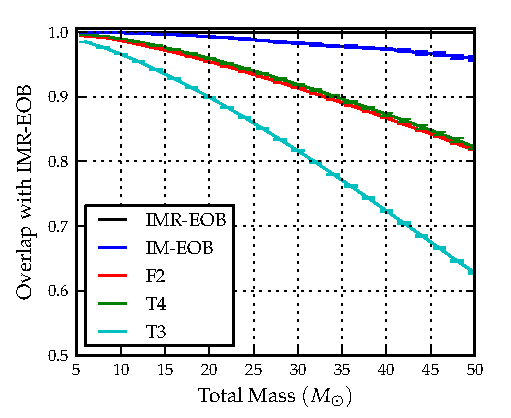
\includegraphics[scale=0.03, clip=false, height=0.28\textheight, width=\columnwidth]{Olaps_q_1_run03.pdf}}                
  \subfigure[$q=2$]{\label{fig:Olapsq2}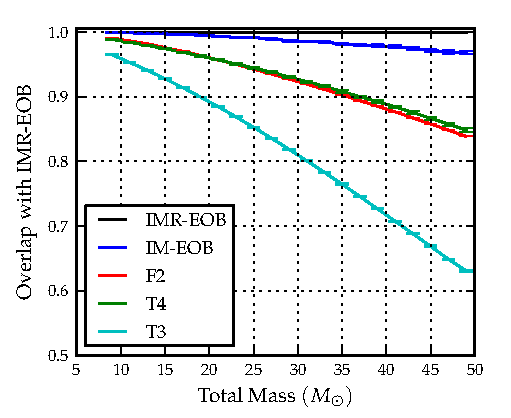
\includegraphics[scale=0.03, clip=false, height=0.28\textheight, width=\columnwidth]{Olaps_q_2_run03.pdf}}
\\ \subfigure[$q=3$]{\label{fig:Olapsq3}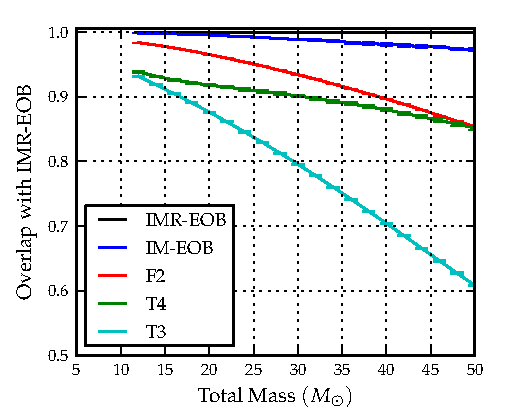
\includegraphics[scale=0.03, clip=false, height=0.28\textheight, width=\columnwidth]{Olaps_q_3_run03.pdf}}
\subfigure[$q=4$]{\label{fig:Olapsq4}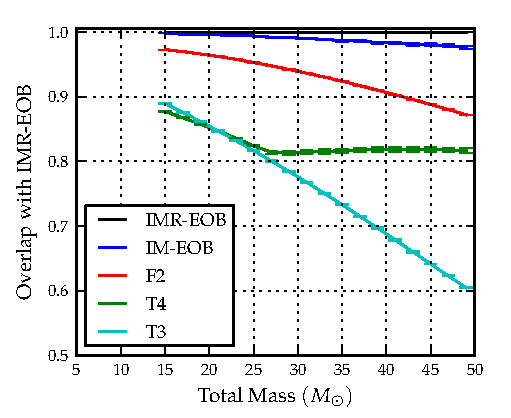
\includegraphics[scale=0.03, clip=false, height=0.28\textheight, width=\columnwidth]{Olaps_q_4_run03.pdf}}
\\ \subfigure[$q=5$]{\label{fig:Olapsq5}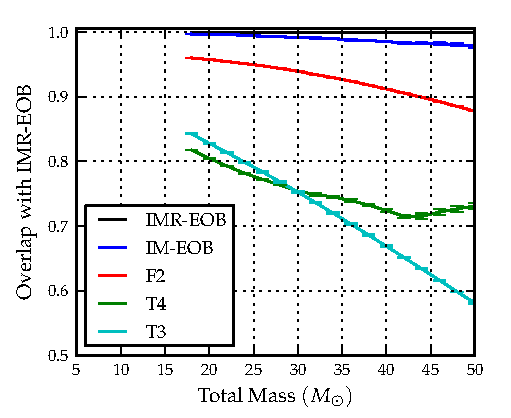
\includegraphics[scale=0.03, clip=false, height=0.28\textheight, width=\columnwidth]{Olaps_q_5_run03.pdf}}
\subfigure[$q=6$]{\label{fig:Olapsq6}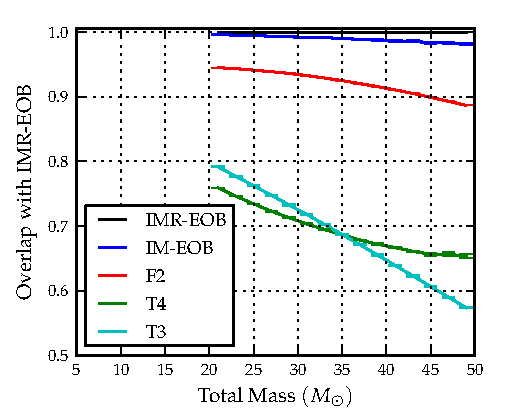
\includegraphics[scale=0.03, clip=false, height=0.28\textheight, width=\columnwidth]{Olaps_q_6_run03.pdf}}
  \caption{Maximized overlaps of different waveform families with EOB. Each subplot is for a different value of mass ratio $q \l(\equiv m_1/m_2\r)$.}
  \label{fig:Olaps}
\end{figure*}

There are a couple of subtle features that were noticed in these figures. 

Firstly, at each value of total mass for a system (for any mass-ratio), we observe numerically small variation in the value of overlaps, of the order$\sim 10^{-3}$. This happens, because, different starting value of phase of the waveforms results in them ending at slightly different points in a wave cycle (illustrated in Fig.\ref{fig:Olapphi0}). And since the amplitude of the waveform is higher during the last few cycles (near the ISCO) than at the beginning, this slight difference towards the end contributes to small numerical fluctuations in overlap values. So, for every value of $(M,q)$, we computed the overlaps for $50$ different values of initial phases, and plotted the mean in Fig.\ref{fig:Olaps}. The variance of the distribution of overlap values at each point is plotted as an errorbar at each data-point.

\begin{figure}
\centering
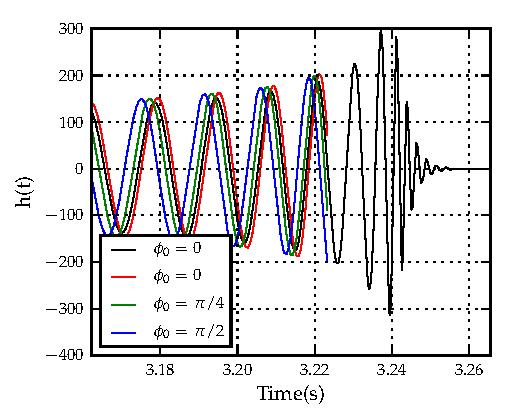
\includegraphics[scale=1.0, clip=false, totalheight=0.3\textheight, width=\columnwidth]{tdwaveform_phi0.pdf}
\caption{\label{fig:Olapphi0}The black waveform is EOBNRv2, and the others are T4 waveforms. The parameters of the system  are $M=44.8M_{\odot},q=1$. The maximized overlap between the EOBNRv2 waveform and T4 waveforms with different initial phases, has a variation of $\backsim1\%$, which is depicted in the errorbars in Fig.\ref{fig:Olaps}}
\end{figure}

Secondly, for asymmetric systems with $q\geq3$, we observe that T4 overlaps don't decrease monotonically with increasing total mass of the system. Above a certain value of total mass, T4 overlaps plateau or start decreasing at a slower rate. This is an artifact of the fact that T4 evolution is slower than EOB waveforms, resulting in the T4 waveform lasting longer than it's EOB counterpart. Fig.\ref{fig:OlapDephasing} depicts this more clearly. The cycles towards the end of the T4 waveform match with the merger chirp of EOB waveform, thus the marked increase in overlaps. As the total mass of the system increases, there are a few competing effects in action. The end-of-inspiral and merger gain relative importance; so the dephasing near the ISCO between the two approximants gains relative importance, and so does the accidental match of T4 cycles with EOB merger-ringdown. These competing effects result in a slower decrease in overlaps/even slight increase in overlaps, as seen in Fig.\ref{fig:Olapsq3}-\ref{fig:Olapsq6}.

\begin{figure*}
  \centering
  \subfigure[$q=1$]{\label{fig:OlapDephasingq1}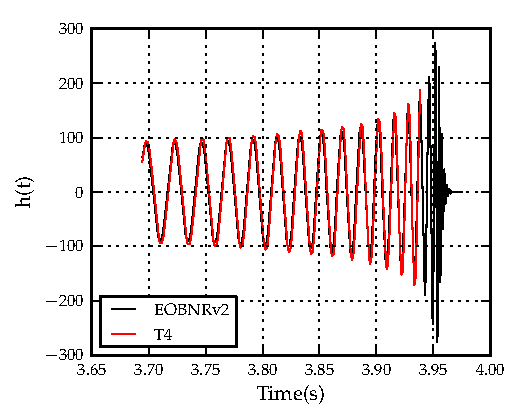
\includegraphics[scale=1.0, clip=true, totalheight=0.28\textheight, width=\columnwidth]{tdwaveform_ISCOshifted_M40_q01.pdf}}                
  \subfigure[$q=4$]{\label{fig:OlapDephasingq4}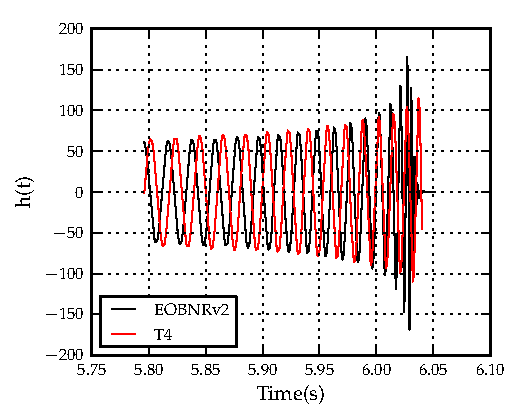
\includegraphics[scale=1.0, clip=true, totalheight=0.28\textheight, width=\columnwidth]{tdwaveform_ISCOshifted_M40_q04.pdf}}
  \caption{The cause for non-steady decline in overlap values, is illustrated in Fig\ref{fig:OlapDephasingq1}. Its the dephasing near the ISCO,  which becomes more important as we increase the total Mass of the system, as it enters LIGO's sensitive band. Also, as $q \l(\equiv m_1/m_2\r)$ increases, we observe dephasing to the extent that the waveforms are more than $2\pi$ out of phase, and hence back into phase towards the end (see Fig\ref{fig:OlapDephasingq4}). These two competing effects account for the change in the rate of decrease of overlaps, as seen in Fig\ref{fig:Olapsq4}.}
  \label{fig:OlapDephasing}
\end{figure*}

This loss in overlap can be translated to loss in effective observation volume. Using the EOB approximant, we calculate the effective distance, the signal from which will be detected with a signal-to-noise ratio of 8. This is initially calculated for an optimally oriented binary (inclination angle = 0), and then scaled to give an average over different sky locations and orientations of the binary. This rescaled effective distance gives us the effective observation volume.

\begin{equation}\label{eq:DeffEOB}
D^{EOB}_{eff} = \dfrac{\sigma^{EOB}}{\rho\l(=8\r)}
\end{equation}

where, $\sigma = \l(h|h\r),h\equiv h^{EOB}$ and $\rho$ is the SNR. However, for other approximants, the effective distance to which we can see binaries is the effective distance we could see to with the exact waveforms scaled by the loss in signal-to-noise ratio due to the inherent inaccuracy of the approximant. This loss in SNR, is approximated by loss in maximized overlap, and so the effective distance to which we can see using other approximants is given by: 

\begin{equation}\label{eq:DeffPN}
D^X_{eff} = D^{EOB}_{eff} \times \l(\hat{h^X}|\hat{h^{EOB}}\r)
\end{equation}

where, $X = \{$T3,T4,F2,EOB without merger-ringdown$\}$; and $h^X$ is the waveform generated using approximant $X$. We get the effective distance averaged over sky-locations and inclination angle $\l(r_{eff}\r)$ by\citep{FinnChernoffDA}:

\begin{align}\label{eq:Veff}
r_{eff} = \dfrac{1}{2.6}D_{eff}\\
V_{eff} = \dfrac{4\pi}{3} r^3_{eff}
\end{align}

where, $(1/2.6)$ is the factor that accounts for different sky locations and orientations of the binary. This effective observation volume, assuming a homogenous distribution of binaries, is directly proportional to observed event rate.

Fig.\ref{fig:VeffsLog} shows variation of the effective observation volume with total mass, for each of the waveform approximants and mass-ratio $q=\{1,2,3,4,5,6\}$. As with the overlap plots in Fig.\ref{fig:Olaps}, the errorbars give the variance because of fluctuations in overlap due to different initial values of phase. And the peculiar trend for Taylor T4, is the same as the trend in Fig.\ref{fig:Olaps}, with the same origin.

\begin{figure*}%[p]
  \centering
  \subfigure[$q=1$]{\label{fig:VeffsLogq1}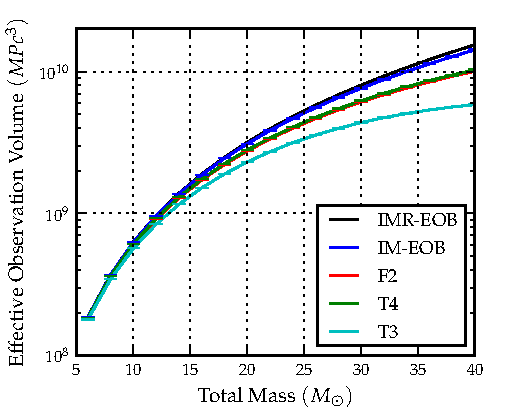
\includegraphics[scale=0.03, clip=false, height=0.28\textheight, width=\columnwidth]{Veffs_logscale_q_1_run03.pdf}}                
  \subfigure[$q=2$]{\label{fig:VeffsLogq2}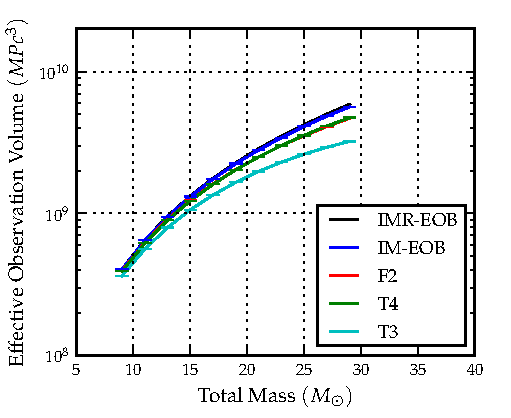
\includegraphics[scale=0.03, clip=false, height=0.28\textheight, width=\columnwidth]{Veffs_logscale_q_2_run03.pdf}}
\\ \subfigure[$q=3$]{\label{fig:VeffsLogq3}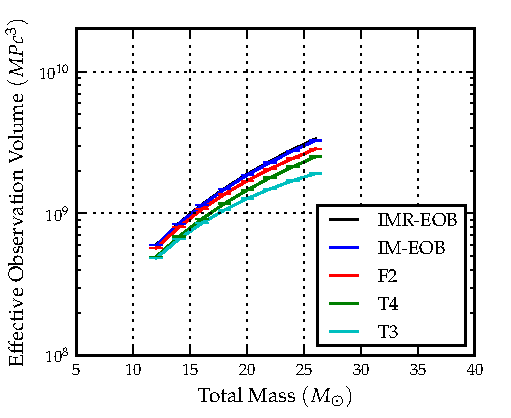
\includegraphics[scale=0.03, clip=false, height=0.28\textheight, width=\columnwidth]{Veffs_logscale_q_3_run03.pdf}}
\subfigure[$q=4$]{\label{fig:VeffsLogq4}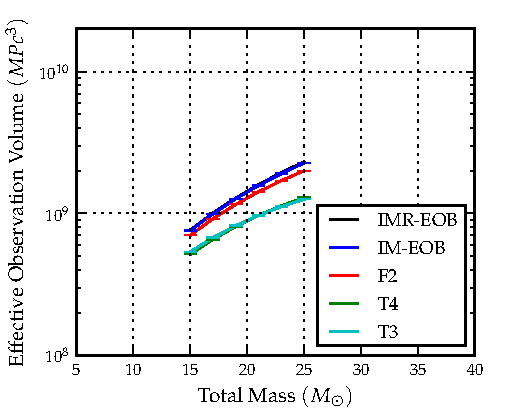
\includegraphics[scale=0.03, clip=false, height=0.28\textheight, width=\columnwidth]{Veffs_logscale_q_4_run03.pdf}}
\\ \subfigure[$q=5$]{\label{fig:VeffsLogq5}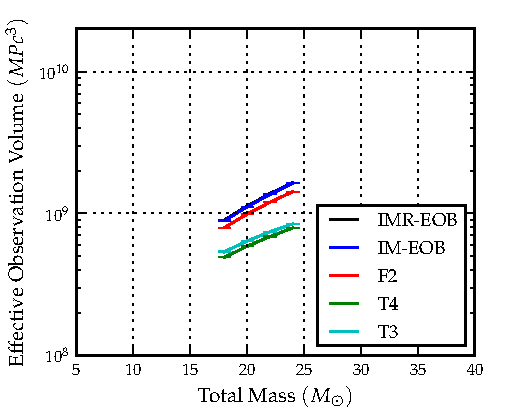
\includegraphics[scale=0.03, clip=false, height=0.28\textheight, width=\columnwidth]{Veffs_logscale_q_5_run03.pdf}}
\subfigure[$q=6$]{\label{fig:VeffsLogq6}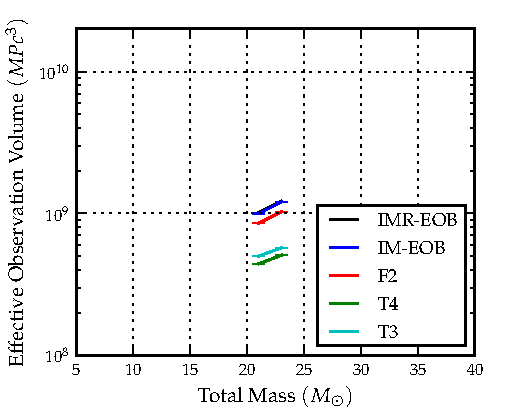
\includegraphics[scale=0.03, clip=false, height=0.28\textheight, width=\columnwidth]{Veffs_logscale_q_6_run03.pdf}}
  \caption{Effective Detection Volume (logarithmic scale), which we would be able to see with different waveform families. Each subplot is for a different value of mass ratio $q \l(\equiv m_1/m_2\r)$.}
  \label{fig:VeffsLog}
\end{figure*}


\begin{figure*}%[p]
  \centering
  \subfigure[$q=1$]{\label{fig:DeffsLinq1}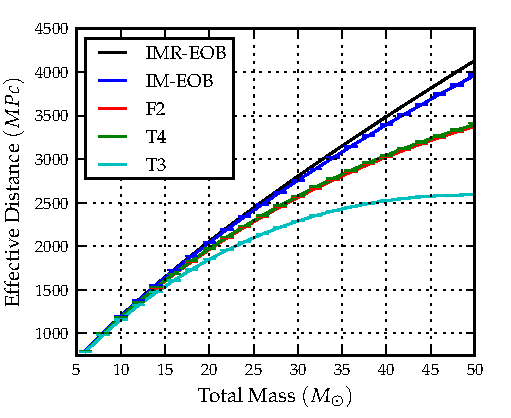
\includegraphics[scale=1.0, clip=true, totalheight=0.28\textheight, width=\columnwidth]{Deffs_linscale_q_1_run03.pdf}}                
  \subfigure[$q=2$]{\label{fig:DeffsLinq2}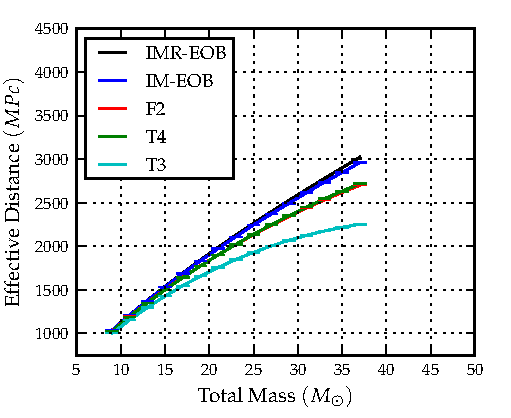
\includegraphics[scale=1.0, clip=true, totalheight=0.28\textheight, width=\columnwidth]{Deffs_linscale_q_2_run03.pdf}}
\\ \subfigure[$q=3$]{\label{fig:DeffsLinq3}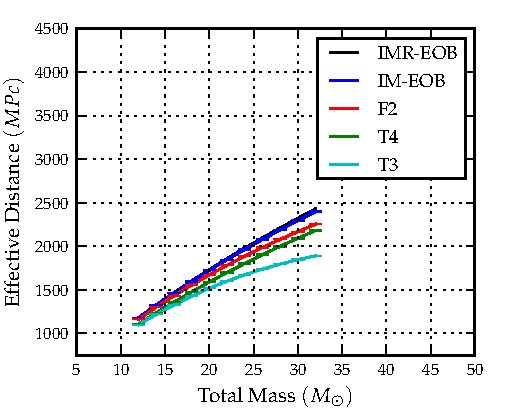
\includegraphics[scale=1.0, clip=true, totalheight=0.28\textheight, width=\columnwidth]{Deffs_linscale_q_3_run03.pdf}}
\subfigure[$q=4$]{\label{fig:DeffsLinq4}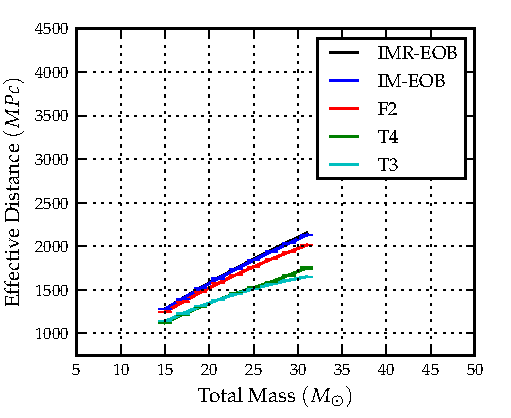
\includegraphics[scale=1.0, clip=true, totalheight=0.28\textheight, width=\columnwidth]{Deffs_linscale_q_4_run03.pdf}}
\\ \subfigure[$q=5$]{\label{fig:DeffsLinq5}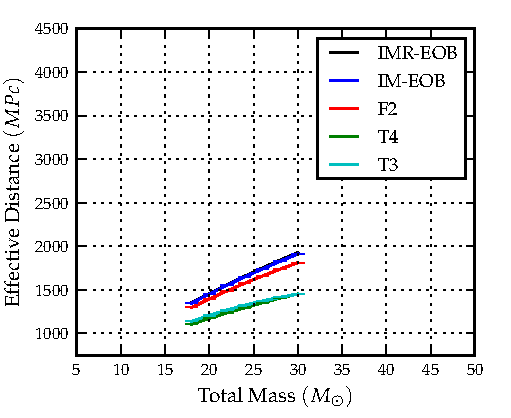
\includegraphics[scale=1.0, clip=true, totalheight=0.28\textheight, width=\columnwidth]{Deffs_linscale_q_5_run03.pdf}}
\subfigure[$q=6$]{\label{fig:DeffsLinq6}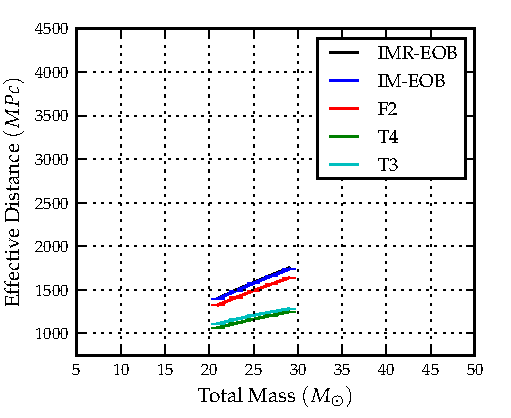
\includegraphics[scale=1.0, clip=true, totalheight=0.28\textheight, width=\columnwidth]{Deffs_linscale_q_6_run03.pdf}}
  \caption{Effective Distances (linear scale), upto which we would be able to see with a particular waveform family. Each subplot is for a different value of mass ratio $q \l(\equiv m_1/m_2\r)$.}
  \label{fig:DeffsLin}
\end{figure*}
 
\begin{figure*}%[p]
  \centering
  \subfigure[$q=1$]{\label{fig:DeffsLogq1}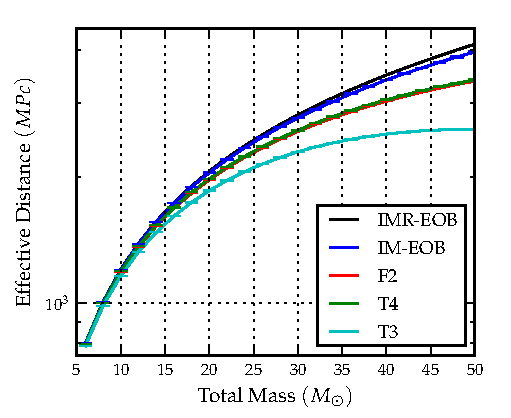
\includegraphics[scale=0.03, clip=false, height=0.28\textheight, width=\columnwidth]{Deffs_logscale_q_1_run03.pdf}}                
  \subfigure[$q=2$]{\label{fig:DeffsLogq2}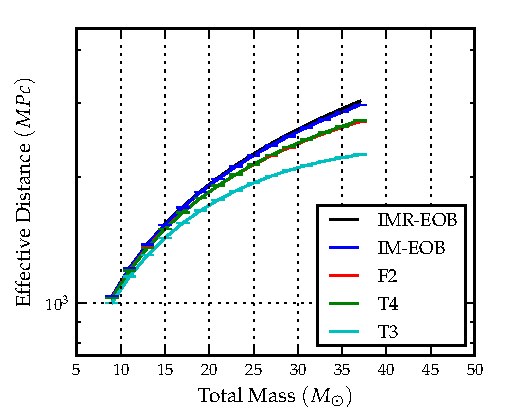
\includegraphics[scale=0.03, clip=false, height=0.28\textheight, width=\columnwidth]{Deffs_logscale_q_2_run03.pdf}}
\\ \subfigure[$q=3$]{\label{fig:DeffsLogq3}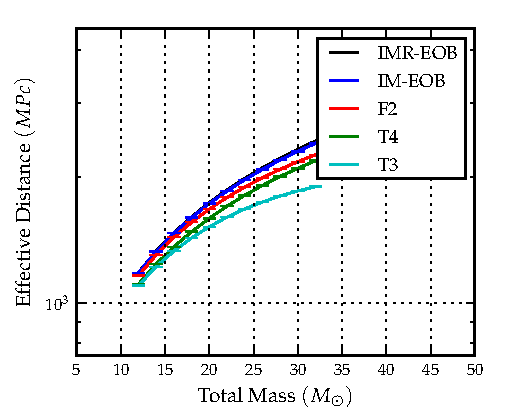
\includegraphics[scale=0.03, clip=false, height=0.28\textheight, width=\columnwidth]{Deffs_logscale_q_3_run03.pdf}}
\subfigure[$q=4$]{\label{fig:DeffsLogq4}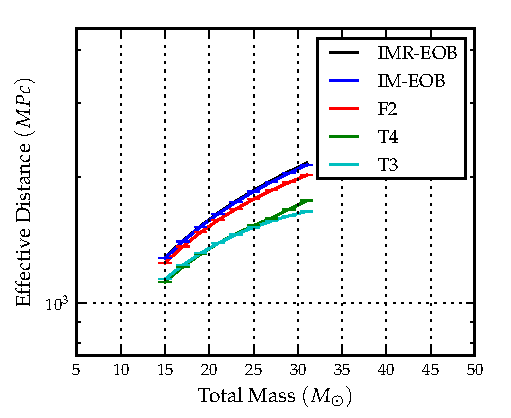
\includegraphics[scale=0.03, clip=false, height=0.28\textheight, width=\columnwidth]{Deffs_logscale_q_4_run03.pdf}}
\\ \subfigure[$q=5$]{\label{fig:DeffsLogq5}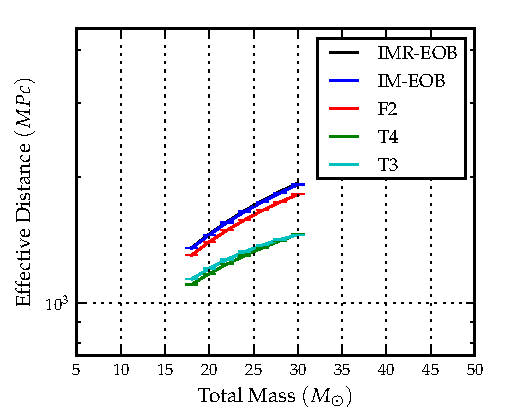
\includegraphics[scale=0.03, clip=false, height=0.28\textheight, width=\columnwidth]{Deffs_logscale_q_5_run03.pdf}}
\subfigure[$q=6$]{\label{fig:DeffsLogq6}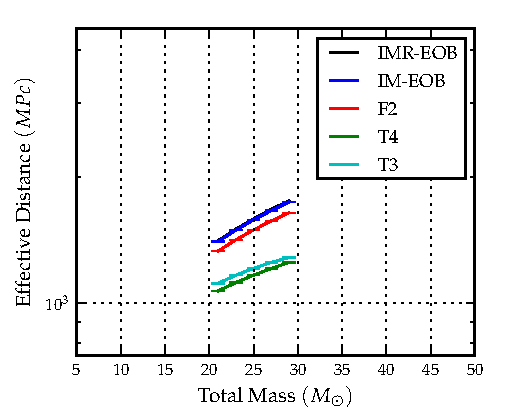
\includegraphics[scale=0.03, clip=false, height=0.28\textheight, width=\columnwidth]{Deffs_logscale_q_6_run03.pdf}}
  \caption{Effective Distances (logarithmic scale), upto which we would be able to see with different waveform families. Each subplot is for a different value of mass ratio $q \l(\equiv m_1/m_2\r)$.}
  \label{fig:DeffsLog}
\end{figure*}

%\begin{figure*}[p]
%  \centering
%  \subfigure[$q=1$]{\label{fig:VeffsLinq1}\includegraphics[scale=1.0, clip=true, totalheight=0.28\textheight, width=\columnwidth]{Veffs_linscale_q_1_run03.pdf}}                
%  \subfigure[$q=2$]{\label{fig:VeffsLinq2}\includegraphics[scale=1.0, clip=true, totalheight=0.28\textheight, width=\columnwidth]{Veffs_linscale_q_2_run03.pdf}}
%\\ \subfigure[$q=3$]{\label{fig:VeffsLinq3}\includegraphics[scale=1.0, clip=true, totalheight=0.28\textheight, width=\columnwidth]{Veffs_linscale_q_3_run03.pdf}}
%\subfigure[$q=4$]{\label{fig:VeffsLinq4}\includegraphics[scale=1.0, clip=true, totalheight=0.28\textheight, width=\columnwidth]{Veffs_linscale_q_4_run03.pdf}}
%\\ \subfigure[$q=5$]{\label{fig:VeffsLinq5}\includegraphics[scale=1.0, clip=true, totalheight=0.28\textheight, width=\columnwidth]{Veffs_linscale_q_5_run03.pdf}}
%\subfigure[$q=6$]{\label{fig:VeffsLinq6}\includegraphics[scale=1.0, clip=true, totalheight=0.28\textheight, width=\columnwidth]{Veffs_linscale_q_6_run03.pdf}}
%  \caption{Effective Detection Volume (linear scale), which we would be able to see with a particular waveform family. Each subplot is for a different value of mass ratio $q \l(\equiv m_1/m_2\r)$.}
%  \label{fig:VeffsLin}
% \end{figure*}
 

Quantitatively, we find that we can use Taylor F2 waveforms, for $M\leq 10M_{\odot}$, with loss in overlap varying from $1.5\%\l(q=1\r)\quad-\quad5\%\l(q=6\r)$. Also, for total mass between $10M_{\odot}$ and $15M_{\odot}$, we can use Taylor F2 waveforms, with the maximum loss in overlap varying from $3\%\l(q=1\r)\quad-\quad5\%\l(q=6\r)$. 

For $q=\{1,2\}$, Taylor T4 has overlaps greater than $0.97$ for total mass less than $15M_{\odot}$. But, as we increase the mass-ratio beyond 2, T4 have much lower overlaps than Taylor F2 approximant $\l(0.95\r)$. So, we can use either Taylor T4 or Taylor F2 for $q=\{1,2\}$, for total mass less than $15M_{\odot}$, with a maximal mismatch of $3\%$. For higher mass-ratios, we can use Taylor F2 for total masses upto $\sim 10M_{\odot}$ with a maximal mismatch of $5\%$ in overlap.

\section{EOB: Data Analysis Study}\label{sec:level1:EOBDA}
The EOB approximant is considered the most accurate in modeling the dynamics of comparable mass binaries, on account of a few reasons. It employs various re-summation methods to make taylor expansions of its metric coefficients and waveform multipoles convergent \citep{PadeAD,ChebyshevResum2006} (or more recently, Ref.\citep{PadeSubDiag2011}). This ensures that these quantities are well modelled near and beyond the ISCO, where the characteristic velocity becomes large enough for the taylor expansions of the afore-mentioned quantities to become inaccurate. It has factors in the expressions for energy flux and waveform multipoles, that capture the non-circularity of the orbits beyond the ISCO. When the binary spirals in past the ISCO, the rate of loss in energy exceeds what the adiabatic approximation predicts, and these factors account for this excess. Also, the model has pseudo-4 PN and higher PN coefficients introduced in the metric coefficients \citep{BuonannoEOBv2Main}. And, all these additional factors have been calibrated against a set of waveforms, extracted from accurate Numerical Relativity simulations \citep{EOBNR01,EOBNRdevel01,EOBNRdevel02,EOBNRdevel03}.

Because of these reasons, we assume that the EOB waveforms accurately model the gravitational waveforms from nature. In this section we compare the Stationary Phase, Taylor T3 and Taylor T4 approximants with the EOB model, for stellar-mass binary black hole systems. This comparitive analysis tells us when these approximants begin to become inaccurate, owing to each approximant's own inherent inaccuracies. With this information, we can deduce the gain in the sensitivity of any match-filtering search that will be done in detector data, if we use the latest EOB model, instead of using the older PN approximants. Also, it will tell us the region of the component-mass space where the older PN approximants model the gravitational wave signal accurately enough for a match-filtering search.

\subsection{Overlap Comparison with PN approximants}\label{sec:level2:PNComparison}

In recent past, studies\citep{CompTemplates2001,CompTemplates2009,DamourF2EOB01,NRPNComparisonBaker2007,NRPNComparisonBoyleetal} have been done to compare different waveform families, and deduce the loss in signal-to-noise ratio that occurs due to the inherent inaccuracies in approximants. The inherent inaccuracy of an approximant might be due to the break-down of the Post-Newtonian expressions for gravitational flux / energy when the expansion parameter $v\l(\equiv (\pi Mf)^{1/3}\r)$ becomes large (towards the end of inspiral); or because of the approximant not being able to capture the merger-ringdown part of the waveform as they are valid only in the regime where the orbits can be approximated as being quasi-circular (i.e. till ISCO).

Ref.\cite{CompTemplates2009} studies the EOB approximant, against Taylor approximants and find that using any of the Taylor approximants up to a total mass of $12M_{\odot}$ results in no more than a $10\%$ loss in event rate for advanced detectors (or equivalently, no more than a $3\%$ loss in aximized overlap). The new EOB model\citep{BuonannoEOBv2Main}, on the other hand, has been tuned to NR simulations for 5 different mass-ratios, and would, in general be expected to have a slightly different phase evolution than its predecessors in the EOB family tree. Also, a better model of the expected power spectral density of advanced LIGO is available. Here, we make overlap comparisons between the Taylor approximants and the EOB approximant.

For this study, we choose a set of mass-ratio ($m_1/m_2$), $q \in\{1,2,3,4,5,6\}$. For each value of $q$, we vary the total Mass of the system, in the limit that the individual component-masses lie in $(3-25)M_{\odot}$. The limits on individual component-masses is in accordance with the expected mass range of stellar-mass black holes.

For each value of $q$ and total Mass ($M$), we compute the maximized overlap between the full inspiral-merger-ringdown (IMR) EOB waveform, and Stationary Phase, Taylor T3 and Taylor T4 waveforms. In addition to these, for each $(q,M)$ pair, we also compute the overlap between the full inspiral-merger-ringdown EOB waveform and the inspiral-merger (IM) EOB waveform. This lets us study the effect of attaching the ringdown to the inspiral-merger part of the EOB waveform. 
\begin{figure*}[htbp]
  \begin{center}
  	\mbox{
  	\subfigure[$\quad q=1$]{\label{fig:Olapsq1}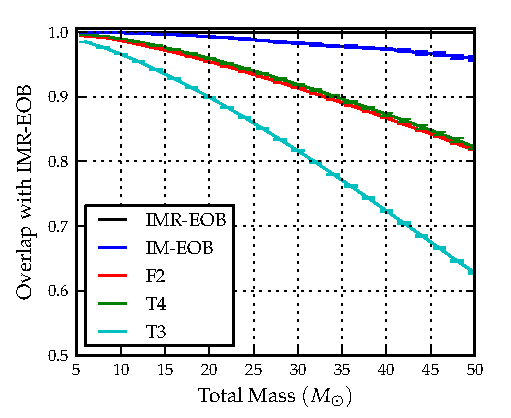
\includegraphics[scale=0.03, clip=false, keepaspectratio=true, width=\columnwidth]{Olaps_q_1_run03.pdf}}                
  	\subfigure[$\quad q=2$]{\label{fig:Olapsq2}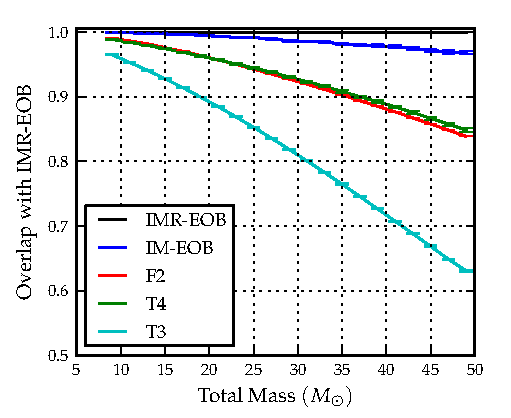
\includegraphics[scale=0.03, clip=false, keepaspectratio=true, width=\columnwidth]{Olaps_q_2_run03.pdf}}
  }
  	\mbox{
 	\subfigure[$\quad q=3$]{\label{fig:Olapsq3}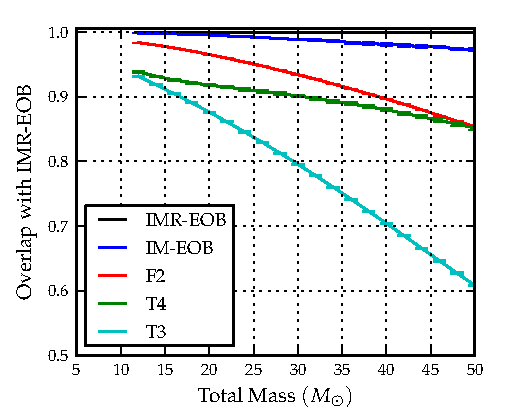
\includegraphics[scale=0.03, clip=false, keepaspectratio=true, width=\columnwidth]{Olaps_q_3_run03.pdf}}
	\subfigure[$\quad q=4$]{\label{fig:Olapsq4}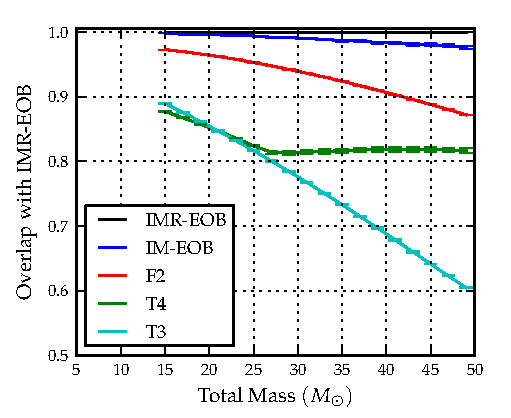
\includegraphics[scale=0.03, clip=false, keepaspectratio=true, width=\columnwidth]{Olaps_q_4_run03.pdf}}
	}
	\mbox{
	\subfigure[$\quad q=5$]{\label{fig:Olapsq5}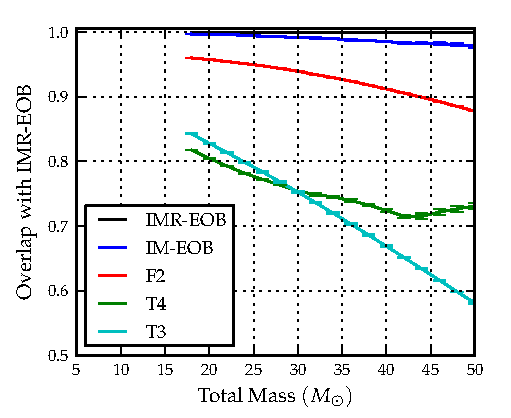
\includegraphics[scale=0.03, clip=false, keepaspectratio=true, width=\columnwidth]{Olaps_q_5_run03.pdf}}
	\subfigure[$\quad q=6$]{\label{fig:Olapsq6}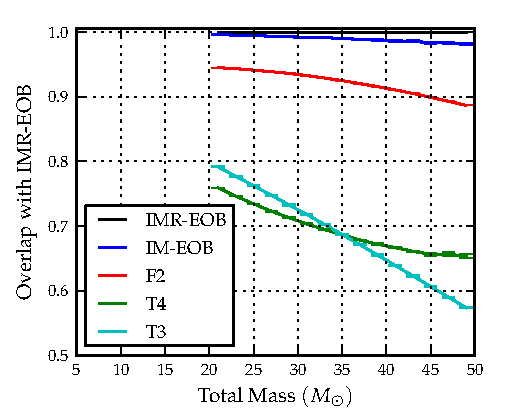
\includegraphics[scale=0.03, clip=false, keepaspectratio=true, width=\columnwidth]{Olaps_q_6_run03.pdf}}
	}
	\caption{This figure shows the maximized overlaps of different PN approximants with the full inspiral-merger-ringdown (IMR) EOB waveforms, as a function of the total mass of the binary. Also shown is the maximized overlap of inspiral-merger (IM) EOB waveforms with the full IMR EOB waveforms.  Each subplot is for a different value of mass ratio $q \l(\equiv m_1/m_2\r)$.}
  \label{fig:Olaps}
  \end{center}
\end{figure*}

Note that, the evolution of each waveform starts from the point where the emitted gravitational wave frequency crosses 15Hz. Also, the EOB waveforms employed in this study (both IMR and IM), have their gravitational flux modelled by summing over 35 leading-order waveform multipoles (i.e. the set of all analytically available multipoles).

The summary of this analysis is illustrated in Fig.\ref{fig:Olaps}. Each subplot in the figure, is for each of the values of $q$, chosen above. We see that for $q\in \{1,2\}$, both the Stationary Phase and the Taylor T4 approximants have high overlaps with the IMR EOB waveforms. These overlaps drop pretty rapidly with increasing total mass of the system, and for systems with total mass above $17M_{\odot}$, the overlap of all PN approximants have dropped below the fiducial value of $0.97$. Also, the overlap of Taylor T3 is consistently worse than Taylor T4, for these values of $q$.

For $q\in \{3,4\}$, we find that none but the Stationary Phase approximant has maximized overlap values $\geq 0.97$. When the total Mass of the system goes above $\sim 18M_{\odot}$, the overlap of Stationary Phase with EOB falls below $0.97$. Taylor T4 and Taylor T3 approximants have overlap values $< 0.97$ in the entire range of total mass for these values of $q$. Taylor T4 does exhibit a peculiar plateauing in overlap values, and this behaviour is investigated in detail, below.

Finally, for $q\in\{5,6\}$, none of the PN approximants have overlaps $>0.97$ with EOB, for any value for total mass of the system.

Apart from this, we observe for each value of $q$, that the overlap of Stationary Phase and Taylor T3 waveforms with EOB waveforms decreases monotonically with increase in total mass of the system. This is consistent with what one naively expects, as with increasing total mass of the system, the waveform terminates at a lower frequency. Since the starting frequency is always the same, with increasing total mass, each waveform has fewer cycles. And with decrease in the number of cycles in the waveform, the merger-ringdown part of the waveform gains relative importance with increase in total mass. Hence, a drop in values of maximized overlap with EOB waveforms, which have merger-ringdown included.

Additionally, the inspiral-merger (IM) EOB waveforms also exhibit a steady decline in overlap values with IMR EOB waveforms. This is also precisely due to the fact that, with increasing total mass of the system, the ringdown gains relative importance. For $q\geq 3$, the overlap of IM EOB waveforms with IMR EOB waveforms never falls below $0.97$. For $q\in\{1,2\}$, the overlap of IM EOB falls below $0.97$ for systems with total masses $>\{42,45\}$ resectively. This indicates that the ringdown has, relatively, more power for symmetric systems, than for asymmetric systems. Since the number of cycles in the inspiral part of the waveform scales with $M^{-1}\eta^{-3/5}$, lower values of $\eta$ leads to waveforms with more inspiral cycles. Thus, as $\eta$ decreases (or $q$ increases), we have waveforms with more cycles in the inspiral part, and the relative power in the ringdown decreases, which agrees with what we observe in Fig.\ref{fig:Olaps}.

For asymmetric systems with $q\geq3$, we observe that T4 overlaps don't decrease monotonically with increasing total mass of the system. Above a certain value of total mass, T4 overlaps plateau or start decreasing at a slower rate or even increase. 

\begin{figure*}[htbp]
  \begin{center}
  	\mbox{
  	\subfigure[$\quad q=1$]{\label{fig:NumCyclesq1}\includegraphics[scale=0.03, clip=false, keepaspectratio=true, width=\columnwidth]{Blank_figure.pdf}}                
  	\subfigure[$\quad q=2$]{\label{fig:NumCyclesq2}\includegraphics[scale=0.03, clip=false, keepaspectratio=true, width=\columnwidth]{Blank_figure.pdf}}
  }
  	\mbox{
 	\subfigure[$\quad q=3$]{\label{fig:NumCyclesq3}\includegraphics[scale=0.03, clip=false, keepaspectratio=true, width=\columnwidth]{Blank_figure.pdf}}
	\subfigure[$\quad q=4$]{\label{fig:NumCyclesq4}\includegraphics[scale=0.03, clip=false, keepaspectratio=true, width=\columnwidth]{Blank_figure.pdf}}
	}
	\mbox{
	\subfigure[$\quad q=5$]{\label{fig:NumCyclesq5}\includegraphics[scale=0.03, clip=false, keepaspectratio=true, width=\columnwidth]{Blank_figure.pdf}}
	\subfigure[$\quad q=6$]{\label{fig:NumCyclesq6}\includegraphics[scale=0.03, clip=false, keepaspectratio=true, width=\columnwidth]{Blank_figure.pdf}}
	}
	\caption{This figure shows the number of cycles in the waveform, starting when the emitted gravitational wave frequency crosses 15Hz. This is shown for each PN approximant, as a function of the total mass of the binary. Each subplot is for a different value of mass ratio $q \l(\equiv m_1/m_2\r)$.}
  \label{fig:NumCycles}
  \end{center}
\end{figure*}
Fig.\ref{fig:NumCycles} shows the number of waveform cycles, for each approximant, in the same range of $q$ and total mass in which the overlap comparisons are made above. We observe that the number of cycles in the waveforms never falls too low for the peculiar-T4-artefact to be because of the waveforms having too few cycles at high masses.

\begin{figure*}[ht]
\centerline{
\includegraphics[scale=1.0, clip=true,keepaspectratio=true, width=\columnwidth]{tdwaveform_ISCOshifted_M30_q01.pdf}\label{fig:OlapDephasingq1}              
\includegraphics[scale=1.0, clip=true, keepaspectratio=true, width=\columnwidth]{tdwaveform_ISCOshifted_M30_q04.pdf}\label{fig:OlapDephasingq4}
}
\caption{The cause for non-steady decline in overlap values, is illustrated in these figures. On the left, we have the late-inspiral cycles of Taylor T4 waveform in red, and the late-inspiral-merger-ringdown cycles of EOB waveform in black, for a binary with $M=30M_{\odot}, q=1$. On the right, we have the late-inspiral cycles of Taylor T4 waveform in red, and the late-inspiral-merger-ringdown cycles of EOB waveform in black, for a binary with the same total mas and $q=4$. In both figures, evolution of both waveforms is started as the emitted gravitational wave frequency crosses 15Hz (at Time = 0s). }
\label{fig:OlapDephasing}
\end{figure*}

It appears that the evolution of dynamics for the T4 approximant is slower (in time) than EOB waveforms. This leads to the T4 waveform lasting longer (in time) than the EOB waveform for the same system. Fig.\ref{fig:OlapDephasing} depicts this more clearly. The dephasing between the two approximants, which becomes more prominent as $q$ increases. We observe dephasing to the extent that the waveforms are more than $2\pi$ out of phase, and hence come back into phase towards the end of T4 inspiral (see Fig\ref{fig:OlapDephasingq4}), which coincides with the merger-ringdown cycles of the EOB waveform. As the total mass of the system increases, and the late inspiral and merger cycles gain relative importance; the dephasing near the ISCO between the two approximants gains relative importance, but so does the accidental match of T4 cycles with EOB merger-ringdown chirp. Thus, with increasing $q$ and total mass, these two effects compete, to result in the kind of plateauing and non-monotonicity we observe in Fig.\ref{fig:VeffsLogq4}-\ref{fig:VeffsLogq6}.

\begin{table}[h]
\caption{\label{tab:maxTotalMassOlap} Maximum total mass of a system, for each value of the mass-ratio, for which the overlap of the respective approximant with full IMR EOB waveform is $\not< 0.97$.}
\begin{ruledtabular}
\begin{tabular}{|m{0.18\columnwidth}| m{0.18\columnwidth}| m{0.18\columnwidth}| m{0.18\columnwidth}| m{0.18\columnwidth}|}
mass-ratio & F2 & T4 & T3 & IM EOB\tabularnewline \hline
1 & 14$M_{\odot}$ & 16$M_{\odot}$ & 8$M_{\odot}$ & 42\tabularnewline \hline
2 & 17$M_{\odot}$ & 15$M_{\odot}$ & - & 45\tabularnewline \hline
3 & 18$M_{\odot}$ & - & - & 50\tabularnewline \hline
4 & 15$M_{\odot}$ & - & - & 50\tabularnewline \hline
5 & - & - & - & 50\tabularnewline \hline
6 & - & - & - & 50\tabularnewline \hline
\end{tabular}
\end{ruledtabular}
\end{table}

\begin{table}[h]
\caption{\label{tab:maxTotalMassOlap} Maximum total mass of a system, for each value of the mass-ratio, for which the overlap of the respective approximant with full IMR EOB waveform is $\not< 0.975$.}
\begin{ruledtabular}
\begin{tabular}{|m{0.18\columnwidth}| m{0.18\columnwidth}| m{0.18\columnwidth}| m{0.18\columnwidth}| m{0.18\columnwidth}|}
mass-ratio & F2 & T4 & T3 & IM EOB\tabularnewline \hline
1 & 14$M_{\odot}$ & 14$M_{\odot}$ & 8$M_{\odot}$ & 38\tabularnewline \hline
2 & 15$M_{\odot}$ & 13$M_{\odot}$ & - & 41\tabularnewline \hline
3 & 16$M_{\odot}$ & - & - & 46\tabularnewline \hline
4 & - & - & - & 49\tabularnewline \hline
5 & - & - & - & 50\tabularnewline \hline
6 & - & - & - & 50\tabularnewline \hline
\end{tabular}
\end{ruledtabular}
\end{table}


\begin{figure}[h]
%\centering
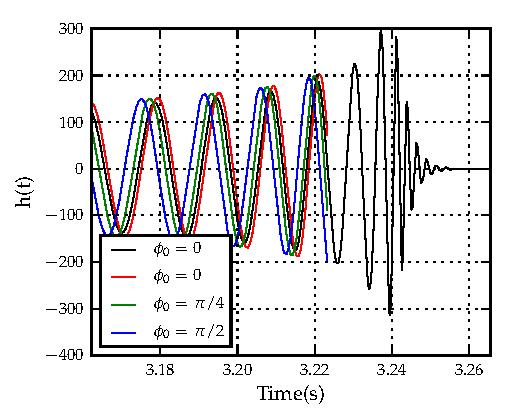
\includegraphics[scale=1.0, clip=false, keepaspectratio=true, width=\columnwidth]{tdwaveform_phi0.pdf}
\caption{\label{fig:Olapphi0}This figure shows parts of 4 waveforms. In black, are the late-inspiral-merger-ringdown cycles of the EOB waveform, for a fiducial binary with $M=44.8M_{\odot},q=1$. Its evolution starts when the gravitationl wave frequency crosses 15Hz (at Time = 0s), and its starting phase is set to 0. In red, green and blue are shown the late-inspiral cycles of the Taylor T4 waveform for the same system. The only difference being, that the initial phase of the three is set to $\{0,\pi/4,\pi/2\}$ respectively. The maximized overlap between the EOB waveform and the T4 waveforms, vary by $\backsim1\%$ between the three values of initial phase (for this fiducial system).}
\end{figure}

There is another small subtle feature in Fig.\ref{fig:Olaps}, that was noticed. At each value of total mass for a system (for any mass-ratio), we observe numerically small variation in the value of overlaps, of the order$\sim 10^{-3}$. This happens, because, different starting value of phase of the waveforms results in them ending at slightly different points in a wave cycle (illustrated in Fig.\ref{fig:Olapphi0}). And since the amplitude of the waveform is higher during the last few cycles (near the ISCO) than at the beginning, this slight difference towards the end contributes to small numerical fluctuations in overlap values. For every $(M,q)$ pair, we computed the overlaps for $50$ different values of initial phases, uniformly sampled in $(0,\pi)$, and plotted the mean in the above-mentioned overlap plots. The variance of the distribution of these numerical fluctuations is plotted as an error-bar at each data-point in Fig.\ref{fig:VeffsLog}.

And, finally, Table\ref{tab:maxTotalMassOlap} gives the maximum values of total mass of a system (for each value of $q$), for which a particular approximant has an overlap $0.97$ with IMR EOB waveforms. We can infer, conservatively, that for stellar-mass black hole binary systems with the total mass $\leq 14M_{\odot}$, and individual component-mass $\geq 3M_{\odot}$, Stationary Phase approximant models the gravitational waveform accurately upto a loss in overlap of $3\%$. Also, below a total mass of $15M_{\odot}$, and $q\leq 2$, Taylor T4 approximant also models the gravitational waveform to the same accuracy. Taylor T3 approximant, is almost uniformly ineffecient in accurately modeling these systems. The accuracy threshold of $3\%$ loss in maximized overlap, is chosen, as it roughly corresponds to a $\sim10\%$ loss in event rate, for match-filtering searches.

\subsection{Gain in Search Sensitivity}\label{sec:level2:GainSearchSens}

The sensitivity of a match-filtering search can be measured in terms of the effective spacial volume, within which all binary systems emitting gravitational radiation will be detected with a signal-to-noise ratio (SNR) $\geq 8$. Specifically, we are concerned with the detection of gravitational radiation from stellar-mass black holes binaries, with individual component-mass ranging in $(3-25)M_{\odot}$. To obtain the effective observation volume, first, the effective observation distance for an optimally oriented system (with inclination angle: $\iota=0$) is calculated. Effective observation distance is the physical distance (in MPc), at which if an optimally oriented binary is located, the match-filter will detect it with a signal-to-noise ratio of 8. Given the effective distance, we can find the actual physical distance at which the binary \textit{could} be located. Effective volume is the volume enclosed by the surface defined by the locus of the possible physical distances (which will have a spatial angular dependence) for a measured effective distance. By definition, all binaries within this spatial volume, will emit gravitaional radiation that will have a signal-to-noise ratio (SNR) $\geq 8$. We can find the radius of a sphere which has the same volume as the effective volume defined above, analytically, which will give us the effective observation volume.

\begin{figure*}%[p]
  \centering
  \subfigure[$q=1$]{\label{fig:VeffsLogq1}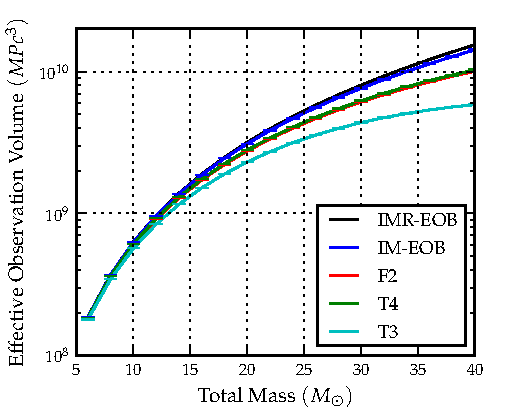
\includegraphics[scale=0.03, clip=false, height=0.28\textheight, width=\columnwidth]{Veffs_logscale_q_1_run03.pdf}}                
  \subfigure[$q=2$]{\label{fig:VeffsLogq2}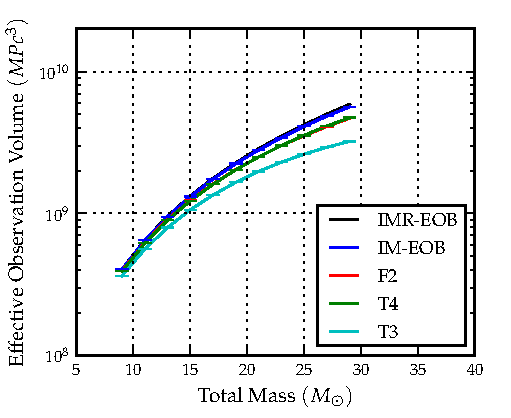
\includegraphics[scale=0.03, clip=false, height=0.28\textheight, width=\columnwidth]{Veffs_logscale_q_2_run03.pdf}}
\\ \subfigure[$q=3$]{\label{fig:VeffsLogq3}\includegraphics[scale=0.03, clip=false, height=0.28\textheight, width=\columnwidth]{Veffs_logscale_q_3_run03.pdf}}
\subfigure[$q=4$]{\label{fig:VeffsLogq4}\includegraphics[scale=0.03, clip=false, height=0.28\textheight, width=\columnwidth]{Veffs_logscale_q_4_run03.pdf}}
\\ \subfigure[$q=5$]{\label{fig:VeffsLogq5}\includegraphics[scale=0.03, clip=false, height=0.28\textheight, width=\columnwidth]{Veffs_logscale_q_5_run03.pdf}}
\subfigure[$q=6$]{\label{fig:VeffsLogq6}\includegraphics[scale=0.03, clip=false, height=0.28\textheight, width=\columnwidth]{Veffs_logscale_q_6_run03.pdf}}
  \caption{Effective Detection Volume (logarithmic scale), which we would be able to see with different waveform families. Each subplot is for a different value of mass ratio $q \l(\equiv m_1/m_2\r)$.}
  \label{fig:VeffsLog}
\end{figure*}


Using the EOB approximant, we calculate the effective distance, the gravitaional wave signal from which will be detected with a signal-to-noise ratio of 8. 
\begin{equation}\label{eq:DeffEOB}
D^{EOB}_{eff} \equiv \dfrac{\sigma^{EOB}}{\rho} = \dfrac{\sigma^{EOB}}{8}
\end{equation}
where, $\sigma^2\equiv\l(h|h\r),h\equiv h^{EOB}$ and $\rho$ is the SNR. However, for other approximants, the effective distance to which a match filtering search can detect using that approximant is the effective distance the same search could detect to with the exact waveforms scaled by the fractional loss in signal-to-noise ratio due to the inherent inaccuracy of the approximant. The \textit{exact} waveform, is taken to be the EOB waveform here. And the fractional loss in SNR, is approximated by loss in maximized overlap between the waveform generated using the particular approximant and that generated using the EOB approximant. So, the effective distance to which match-filtering searches can detect signals to, in advanced LIGO data, using approximant $X$, is given by: 
\begin{equation}\label{eq:DeffPN}
D^X_{eff} = D^{EOB}_{eff} \times \l(\hat{h^X}|\hat{h^{EOB}}\r)
\end{equation}
where, $X\in\{$T3,T4,F2,IM-EOB$\}$; and $h^X$ is the waveform generated using approximant $X$. The effective distance is equal to the physical distance for an optimally oriented binary (inclination angle: $\iota = 0$), but for non-optimally oriented binaries, the physical distance is smaller by a factor governed by the sensitivity patterns of the detector.
\begin{equation}
D_{eff} = \dfrac{D_{phys}}{\sqrt{F^2_+\l(1+\cos^2\iota\r)/4 + F^2_{\times}\cos^2\iota}}
\end{equation}
where, 
\begin{align*}\nonumber
F_+ = \dfrac{1}{2}(1+\cos^2\theta)\cos2\Phi \cos2\Psi - \cos\theta \sin2\Phi \sin2\Psi\\
F_+ = \dfrac{1}{2}(1+\cos^2\theta)\cos2\Phi \sin2\Psi + \cos\theta \sin2\Phi \cos2\Psi
\end{align*}
are the antenna patterns of the detector\citep{SathyaSchutzLRR}, and $\{\theta,\Phi,\Psi\}$ are the 3 Euler angles that take the frame in which the binary is in the x-y plane, and its angular momentum is pointing towards z-axis; to the frame whose x and y axes rest along LIGO's arms, z-axis points outwards from the surface of Earth.

To get the effective volume, we need to find the radius of the sphere, whose volume equals the volume of space that encapsulates all sources that will be detectable with $\rho \geq 8$. Ref.\citep{FinnChernoffDA} calculates this to be (Eq.(5.1,5.2)):
\begin{align}\nonumber
R_{eff} = & r_0 \left[3\int_0^{\infty} dx x^2 P(\rho^2(x)\geq\rho_0^2) \right]^{1/3}\\
\equiv & r_0 \left[3\int_0^{\infty} dx x^2 P(\Gamma\geq x^2) \right]^{1/3}
\end{align}
where, $r_0$ is a fiducial distance, defined in Eq.(5.2a) of Ref.\citep{FinnChernoffDA}:
\begin{align}\nonumber
r_0 \equiv & \l(\dfrac{5M^{5/3}\eta f_{7/3}}{96\pi^{4/3}\rho_0^2} \r)^{1/2}\\
f_{7/3} = &  \int_0^{\infty} df \left[f^{7/3} S_n(f) \right]^{-1}\\
\Gamma = & 16\left[F^2_+\l(1+cos^2\iota\r)/4 + F^2_{\times}cos^2\iota \right]
\end{align}
and $\Gamma\in [0,16]$. Now, if all the sources were optimally oriented, $\Gamma = 16$ always, and $R_{eff}(=R_{eff}^{opt})$ for such a distribution would be equal to $D_{eff}$.
\begin{align}\nonumber
R^{opt}_{eff} = & r_0 \left[3\int_0^{\infty} dx x^2 P(\Gamma > x^2) \right]^{1/3}\\ \nonumber
= & r_0 \left[3\int_0^{4} dx x^2 \right]^{1/3}\\ 
= & 4 r_0
\end{align}
On the other hand, if they are all isotropically distributed in space, 
\begin{align}\nonumber\label{eq:RisoIntegral}
R^{iso}_{eff} = & r_0 \left[3\int_0^{\infty} dx x^2 P(\Gamma > x^2) \right]^{1/3}\\
= & (3\times 1.84)^{1/3} r_0
\end{align}
The last integral has been numerically evaluated in Ref.\citep{FinnChernoffDA}. So, the effective volume will be:
\begin{equation}\label{eq:Veff}
V_{eff} = \dfrac{4\pi}{3} R^3_{eff}
\end{equation}
where, 
\begin{align}\nonumber
R_{eff} \equiv & R^{iso}_{eff}\\ \nonumber
= & \dfrac{(3\times 1.84)^{1/3}}{4} R^{opt}_{eff}\\
= & \dfrac{1}{2.26} R^{opt}_{eff}\\ \nonumber
= & \dfrac{1}{2.26} D_{eff}
\end{align}
Note, that this effective observation volume is proportional to the event rate, if we assume that binary systems are isotropically distributed in the entire volume. In the calculations above, we've already tacitly assumed that, while using the integral in Eq.\eqref{eq:RisoIntegral} evaluated in Ref.\citep{FinnChernoffDA}.

Fig.\ref{fig:VeffsLog} shows the variation of the effective observation volume with total mass, for each of the waveform approximants, for certain values of mass-ratio $q=\{1,2,3,4,5,6\}$. For $q\geq 3$, we can observe that using Taylor T4 or Taylor T3 approximants leads to visibly large reduction in the effective observation volume. All the PN approximants seem to be effective in match-filtering waveforms from equal-mass binary systems, with total mass below $\sim 14M_{\odot}$. But as soon as one moves towards asymmetric binaries, the PN approximants rapidly lose their efficiency in searching for waves from such systems. Quantitatively, what we observe has already been summarized in Table\ref{tab:maxTotalMassOlap}. Stationary Phase approximant can be used to match-filter signals from binary systems with individual component-mass above $3M_{\odot}$ and total mass below $14M_{\odot}$, with $<10\%$ loss in effective observation volume, and hence the event rate. However, above a total mass of $14M_{\odot}$, using any of the PN approximants leads to $>10\%$ loss in effective observation volumes for more asymmetric systems.

Similar to Fig.\ref{fig:Olaps}, in the effective observation volume numbers, we observe very small numerical fluctuations. The cause of these is the same as described in Sec.\ref{sec:level2:PNComparison}, and just like in Fig.\ref{fig:Olaps}, the variance of these fluctuations are plotted as errorbars in Fig.\ref{fig:VeffsLog}. Also, the strange behaviour of the T4 waveforms for more asymmetric systems, is also carried over to these figures, and have the same cause as described in Sec.\ref{sec:level2:PNComparison}.


%\FloatBarrier
\section{Detection Seach: Optimally Using Waveform Approximants}\label{sec:level1:DetectionSeach}

In this section, we try to determine the region in the component-mass space where we can effectively use the Stationary Phase waveforms to perform a detection search, and in the region where its just more effective to use the Effective-One-Body waveforms.

\subsection{Template Bank: Sufficiency of the 2PN metric}\label{sec:level2:TemplateBank}

Take 2 neighbouring points on the component-mass space, and generate the gravitational waveforms for these systems, using the Stationary Phase approximant at 2PN. The template placement metric gives us the overlap between these two waveforms, given just the 2 sets of component-mass values. Using this, we can efficiently pack any region in the component-mass space with a set of points called the \textit{bank}, in such a way that the overlap between the waveform generated for any component-mass values in the region and at least one waveform in the bank will be above a pre-specified threshold. This threshold on minimum overlap will be called the \textit{minimal match}.

In this section, we try to analyze the sufficiency and efficiency of the 2PN metric that is used to gauge the overlap between 2 nearby points on the component-mass space. This was developed in Ref.\citep{SathyaMetric2PN,OwenTemplateSpacing,SathyaBankPlacementTauN}, and the algorithm to use the metric to create a bank with a prespecified minimal match was developed in Ref.\citep{BabaketalBankPlacement}. 

This allows us to restrict the loss in signal-to-noise ratio because of using a discrete set of templates to search for the gravitational-wave signals in detector data, in a quantitative way.

Now, to test if the bank population using this metric is efficient for a particular waveform approximant, we will employ the following strategy: First, generate a bank that covers the SMBHB component-mass region, with a known intended minimal match. Then, do a Monte-Carlo simulation with points distributed uniformly over the entire region in the component-mass space. For each point, we generate the waveform  using that particular approximant, and compute its overlaps with waveforms generated for every point in the entire bank - using the same approximant. Then we just store the maximum of all these values. If the set of these values has values below the minimal match that was specified to create the bank, then we conclude that the bank has not covered the entire region sufficiently for that particular waveform approximant.

Note, that the term \textit{overlap}, here, means the \textit{maximized overlap}, as defined in Sec.\ref{sec:level1:Overlaps}.

\subsubsection{Stationary Phase Waveforms}

To begin with, as a consistency check for this procedure, we do a Monte-Carlo simulation using 2PN Stationary Phase waveforms. A hexagonal template bank is created with an intended minimal match of .97, 
coverage between $3 -20 M_{\odot}$, using the ZERO\_ DET\_ HIGH\_ P aLIGO PSD. A Monte-Carlo simulation is performed by generating 100,000 signals that are randomly chosen and distributed uniformly between component masses $3 -20 M_{\odot}$. The overlap, maximized over time and phase, of each signal waveform is calculated for each template, and the largest overlap over the entire template bank is kept for each signal waveform. 

The results are shown in Fig.[\ref{fig:taylorf2-25PN-hist}] and Fig.[\ref{fig:taylorf2-25PN-bank}]. For Stationary Phase at 2PN the template bank highly overcovers the space, provided a .99 minimal match bank. This is the approximant it was designed for, and it seems to cover the region completely, to the extent of overcovering it. 

Next, the bank is analysed by examining the effectiveness of the metric placement for Stationary Phase waveforms at 3.5PN order. The results are shown in Fig.[\ref{fig:taylorf2-35PN-hist}] and Fig.[\ref{fig:taylorf2-35PN-bank}]. At 3.5PN the coverage exceeds .98 minimal match. The overcoverage seems to be the greatest near the equal mass line, for both the PN orders.

The bank placement covers the component-mass space efficiently, to the extent of overcovering it. 
\begin{figure}[h]
%\centering
\includegraphics[scale=0.04, clip=false, totalheight=0.3\textheight]{taylorf2-2pn-hist.pdf}[h]
\caption{\label{fig:taylorf2-25PN-hist} Distribution of overlap values between Taylor F2 2.5PN waveforms
 in a hexagonal bank with a .97 minimal match, placed according to the Owen-Sathya metric, and Taylor F2 2.5PN
  waveforms that are distributed uniformly between component masses $3 -20 M_{\odot}$.}
\end{figure}

\begin{figure}[h]
%\centering
\includegraphics[scale=0.04, clip=false, totalheight=0.3\textheight]{taylorf2-2pn-bank.pdf}
\caption{\label{fig:taylorf2-25PN-bank} Overlap values of Taylor F2 2.5PN waveforms that are distributed 
uniformly between component masses $3 -20 M_{\odot}$. The color of each point represents the overlap value 
maximized over time, phase, and the template bank. The template bank contains Taylor F2 2.5PN waveforms placed 
according to the Owen-Sathya metric with hexagonal arrangement and a .97 minimal match.}
\end{figure}

\begin{figure}
%\centering
\includegraphics[scale=0.04, clip=false, totalheight=0.3\textheight]{taylorf2-35pn-hist.pdf}
\caption{\label{fig:taylorf2-35PN-hist}Distribution of overlap values between Taylor F2 3.5PN waveforms
in a hexagonal bank with a .97 minimal match, placed according to the Owen-Sathya metric, and Taylor F2 3.5PN
 waveforms that are distributed uniformly between component masses $3 -20 M_{\odot}$.}
\end{figure}

\begin{figure}
%\centering
\includegraphics[scale=0.04, clip=false, totalheight=0.3\textheight]{taylorf2-35pn-bank.pdf}
\caption{\label{fig:taylorf2-35PN-bank}Overlap values of Taylor F2 3.5PN waveforms that are distributed uniformly
 between component masses $3 -20 M_{\odot}$. The color of each point represents the overlap value maximized over 
 time, phase, and the template bank. The template bank contains Taylor F2 3.5PN waveforms placed according to the
  Owen-Sathya metric with hexagonal arrangement and a .97 minimal match.}
\end{figure}

%We begin the bank's analysis by examining the effectiveness of the metric placement for Taylorf2 waveforms at 3.5PN orders. 
%The results are shown in Fig.[\ref{fig:taylorf2-35PN-hist}]. For taylor F2 at 2PN 
%the template bank highly overcovers the space, provided a .99 minimal match bank. At 3.5PN the coverage exceeds .98 minimal match. 
%The overcoverage is greatest near the equal mass line.  


\subsubsection{Effective-One-Body Waveforms}

\begin{figure}
%\centering
\includegraphics[scale=0.04, clip=false, totalheight=0.3\textheight]{eobnr-hist.pdf}
\caption{\label{fig:eobnr-hist}Distribution of overlap values between EOBNR waveforms in a hexagonal bank with a .97 minimal match, placed according to the Owen-Sathya metric, and EOBNR waveforms that are distributed uniformly between 
component masses $3 -20 M_{\odot}$.}
\end{figure}

\begin{figure}
%\centering
\includegraphics[scale=0.04, clip=false, totalheight=0.3\textheight]{eobnr-bank.pdf}
\caption{\label{fig:eobnr-bank}Overlap values of EOBNR waveforms that are distributed uniformly between component  masses $3 -20 M_{\odot}$. The color of each point represents the overlap value maximized over time, phase, and the template bank. The template bank contains EOBNR waveforms placed according to the Owen-Sathya metric with hexagonal
  arrangement and a .97 minimal match.}
\end{figure}

\begin{figure}
%\centering
\includegraphics[scale=0.04, clip=false, totalheight=0.3\textheight]{eob98hist.pdf}
\caption{\label{fig:eobnr98-hist}Distribution of overlap values between EOBNR waveforms in a hexagonal bank with a .98 minimal match, placed according to the Owen-Sathya metric, and EOBNR waveforms that are distributed uniformly between 
component masses $3 -20 M_{\odot}$.}
\end{figure}

\begin{figure}
%\centering
\includegraphics[scale=0.04, clip=false, totalheight=0.3\textheight]{eob98bank.pdf}
\caption{\label{fig:eobnr98-bank}Overlap values of EOBNR waveforms that are distributed uniformly between component masses $3 -20 M_{\odot}$. The color of each point represents the overlap value maximized over time, phase, and the template bank. The template bank contains EOBNR waveforms placed according to the Owen-Sathya metric with hexagonal arrangement and a .98 minimal match.}
\end{figure}

We examine the ability of the metric to create a bank accurate for EOB waveforms. The result is shown in Fig.[\ref{fig:eobnr-hist}]. The metric, with an intended minimal match of .97, provides a minimal match of .94, as is apparent in Fig.[\ref{fig:eobnr-hist}]. Clearly, this is not sufficient to generate a bank with a minimal match of 0.97.

So, we increase the intended minimal match of the bank to 0.98, to see if the thence generated bank has a minimal match of 0.97 (which we require for detection searches). In Fig.[\ref{fig:eobnr98-bank}] and Fig.[\ref{fig:eobnr98-hist}] we can look at the effect of doing so. It is observed that there is some improvement, but the bank still has an actual minimal match of 0.96.

Taking the next step, we generate a bank with an intended minimal match of 0.99. Fig.[] and [] show the effect of doing so, and now the  bank seems to have an actual minimal match of 0.97. Thus, to generate a bank of EOB templates with a minimal match of 0.97, we must use a bank created with an intended minimal match of 0.99.

\subsection{Effectualness of Taylor approximants: Where can they be used?}

\subsubsection{EOBNR vs EOB}

\begin{figure}
%\centering
\includegraphics[scale=0.04, clip=false, totalheight=0.3\textheight]{eobeobnr-hist.pdf}
\caption{\label{fig:eobeobnr-hist}Distribution of overlap values between EOB waveforms in a hexagonal bank with a .97
 minimal match, placed according to the Owen-Sathya metric, and EOBNR waveforms that are distributed uniformly between 
 component masses $3 -20 M_{\odot}$.}
\end{figure}

\begin{figure}
%\centering
\includegraphics[scale=0.04, clip=false, totalheight=0.3\textheight]{eobeobnr-bank.pdf}
\caption{\label{fig:eoboebnr-bank}Overlap values of EOBNR waveforms that are distributed uniformly between component 
masses $3 -20 M_{\odot}$. The color of each point represents the overlap value maximized over time, phase, and the
 template bank. The template bank contains EOB waveforms placed according to the Owen-Sathya metric with hexagonal arrangement
  and a .97 minimal match.}
\end{figure}

\subsubsection{EOBNR vs Taylor T4}


\subsubsection{EOBNR vs SPA}

%\FloatBarrier
%\section{Higher Order Modes in the Waveform}
%How does including higher order modes in $h_{l,m}$ affect the results?
%\FloatBarrier
\section{Conclusion}\label{sec:level1:Conclusion}

A systematic overlap study of various PN approximants against the EOB approximant, tells us that, for stellar-mass black hole binary systems with individual component mass $>3M_{\odot}$ and total mass $\leq M_{\odot}$, the Stationary Phase approximant models the waveforms accurately enough to have a maximal mismatch of $3\%$ with respective EOB waveforms. Other Taylor waveforms attain the same accuracy threshold to much lower total mass limits. T4 is found accurate in $M<10M_{\odot}$ region, while T3 in the $M<8M_{\odot}$ region. 

Also, in the component-mass region described above $(M_1,m_2>3M_{\odot};M\leq 14M_{\odot})$, it was observed that the Stationary Phase approximant can be used in match-filtering searches with $<10\%$ loss in event observation rate. Match-filtering searches filter detector data in the frequency domain, and a major computational cost is due to the fourier-transform of time-domain waveforms to frequency-domain. Using Stationary Phase waveforms saves a considerable amount of computational effort. Also, the component-mass region that this approximant is found accurate in, has the highest density of points, when one uses the gridded bank of waveforms, designed in Ref.\citep{SathyaMetric2PN}. Thus, we find that this approximant is valid in the component-mass region where the benefit of being able to use it are twofold.

% If in two-column mode, this environment will change to single-column
% format so that long equations can be displayed. Use
% sparingly.
%\begin{widetext}
% put long equation here
%\end{widetext}

% figures should be put into the text as floats.
% Use the graphics or graphicx packages (distributed with LaTeX2e)
% and the \includegraphics macro defined in those packages.
% See the LaTeX Graphics Companion by Michel Goosens, Sebastian Rahtz,
% and Frank Mittelbach for instance.
%
% Here is an example of the general form of a figure:
% Fill in the caption in the braces of the \caption{} command. Put the label
% that you will use with \ref{} command in the braces of the \label{} command.
% Use the figure* environment if the figure should span across the
% entire page. There is no need to do explicit centering.

% \begin{figure}
% \includegraphics{}%
% \caption{\label{}}
% \end{figure}

% Surround figure environment with turnpage environment for landscape
% figure
% \begin{turnpage}
% \begin{figure}
% \includegraphics{}%
% \caption{\label{}}
% \end{figure}
% \end{turnpage}

% tables should appear as floats within the text
%
% Here is an example of the general form of a table:
% Fill in the caption in the braces of the \caption{} command. Put the label
% that you will use with \ref{} command in the braces of the \label{} command.
% Insert the column specifiers (l, r, c, d, etc.) in the empty braces of the
% \begin{tabular}{} command.
% The ruledtabular enviroment adds doubled rules to table and sets a
% reasonable default table settings.
% Use the table* environment to get a full-width table in two-column
% Add \usepackage{longtable} and the longtable (or longtable*}
% environment for nicely formatted long tables. Or use the the [H]
% placement option to break a long table (with less control than 
% in longtable).
% \begin{table}%[H] add [H] placement to break table across pages
% \caption{\label{}}
% \begin{ruledtabular}
% \begin{tabular}{}
% Lines of table here ending with \\
% \end{tabular}
% \end{ruledtabular}
% \end{table}

% Surround table environment with turnpage environment for landscape
% table
% \begin{turnpage}
% \begin{table}
% \caption{\label{}}
% \begin{ruledtabular}
% \begin{tabular}{}
% \end{tabular}
% \end{ruledtabular}
% \end{table}
% \end{turnpage}

% Specify following sections are appendices. Use \appendix* if there
% only one appendix.
%\appendix
%\section{}
%\FloatBarrier
% If you have acknowledgments, this puts in the proper section head.
\begin{acknowledgments}
We thank NSF grants PHY-1040231 and PHY-0600953, for support with the computational resources needed for this work.
\end{acknowledgments}

% Create the reference section using BibTeX:
\bibliography{bank_effectualness_study}

\end{document}
%
% ****** End of file apstemplate.tex ******

